\documentclass[12pt,openany]{book}

%PACKAGES%
\usepackage[inner=23mm, outer=18mm, top=23mm, bottom=28mm, papersize={154mm, 216mm}]{geometry}
\usepackage{graphicx}
\usepackage{fontspec}
\usepackage{enumitem}
\usepackage{sectsty}
\usepackage[]{titlesec}
% \usepackage{verse}
\usepackage{fix-cm}%font size
\usepackage{multirow}%tables
\usepackage{array}%tables
\usepackage[hyphens]{url}
\usepackage{tocloft}
\usepackage{soulutf8}
\usepackage{marginnote}
\usepackage[french]{babel}
\usepackage[document]{ragged2e}
\usepackage{xcolor}
\usepackage{wrapfig}

\graphicspath{ {../images/} }

%this snippet of code is a bit of a hack to allow line break after em-dash (http://tex.stackexchange.com/questions/62800/lualatex-and-line-breaks-after-em-dashes)
\catcode`\—=13
\protected\def—{\unskip\textemdash\allowbreak}

%TABLE OF CONTENTS%
\renewcommand*{\cfttoctitlefont}{\Secfont\Large}%use tocloft
%TABLE OF CONTENTS%

%LINESPACE% SETS LINESPA\caps{ce}
\usepackage{setspace}
\setstretch{1.15}
%LINESPACE%

%FONTS% These are the normal SC fonts. We have a ``light'' skolar, too. 
\setmainfont[Numbers=OldStyle]{Alegreya}
\setsansfont[Scale = MatchLowercase]{Alegreya Sans}
\setmonofont{Alegreya}

\newfontfamily\Chapfont[ItalicFont=Alegreya Sans Italic]{Alegreya Sans}
\chapterfont{\Chapfont\LARGE\centering\mdseries\setstretch{1}}
\newfontfamily\Secfont[Numbers=OldStyle]{Alegreya Sans Medium}
\sectionfont{\Secfont\mdseries\large\setstretch{1}}
\newfontfamily\quotefont{Alegreya Sans}
\AtBeginEnvironment{quote}{\quotefont\small}

% Adjust sectional unit title fonts in ToC
\renewcommand{\cftchapfont}{\sffamily}
\renewcommand{\cftsecfont}{\sffamily}

\hyphenpenalty=5000

%HEADER% 
\setlength{\headheight}{15pt}
\renewcommand{\chaptermark}[1]{\markboth{\thechapter.\ #1}{}}
\renewcommand{\sectionmark}[1]{\markright{\thesection\ #1}}

%HANGING LEFT%
\newcommand*{\vleftofline}[1]{\leavevmode\llap{#1}}
%HANGINGLEFT%

\definecolor{light-gray}{gray}{0.9}
\renewcommand\fbox{\fcolorbox{darkgray}{light-gray}}

\setlength{\fboxsep}{1em}

%WIDOWS & ORPHANS% 
\widowpenalty=10000
\clubpenalty=10000
%WIDOWS & ORPHANS%

% make margins of quotes smaller so it fits better on the pages for french
\renewenvironment{quote}{%
  \list{}{%
    \leftmargin-0.1cm   % this is the adjusting screw
    \rightmargin\leftmargin
  }
  \item\relax
}
{\endlist}

%Applies various subtle improvements in typography. Use default.
\usepackage{microtype}
\frenchspacing

\usepackage[unicode, hidelinks, pdfauthor={Rainbodhi}, pdftitle={Accueillir l’Arc-en-Ciel}, pdfsubject={Bouddhisme}, pdfkeywords={Bouddhisme, LGBTIQA+, queer, transgenre, lesbienne, gay, bisexuel, intersexe, discrimination}, pdfproducer={LuaTeX  beta-0.70.1}, pdfcreator={LaTeX2e}]{hyperref}

%DOCUMENT INFO. NOT USED IN TEXT.%
\title{Accueillir l’Arc-en-Ciel}
\author{Un guide pour l’inclusion de la communauté \mbox{LGBTQIA+} à l’intention des bouddhistes}
\date{}
\begin{document}

\frontmatter

\newgeometry{margin=0pt}

\begin{figure}[ht]
    \centering
    \makebox[0pt]{%
    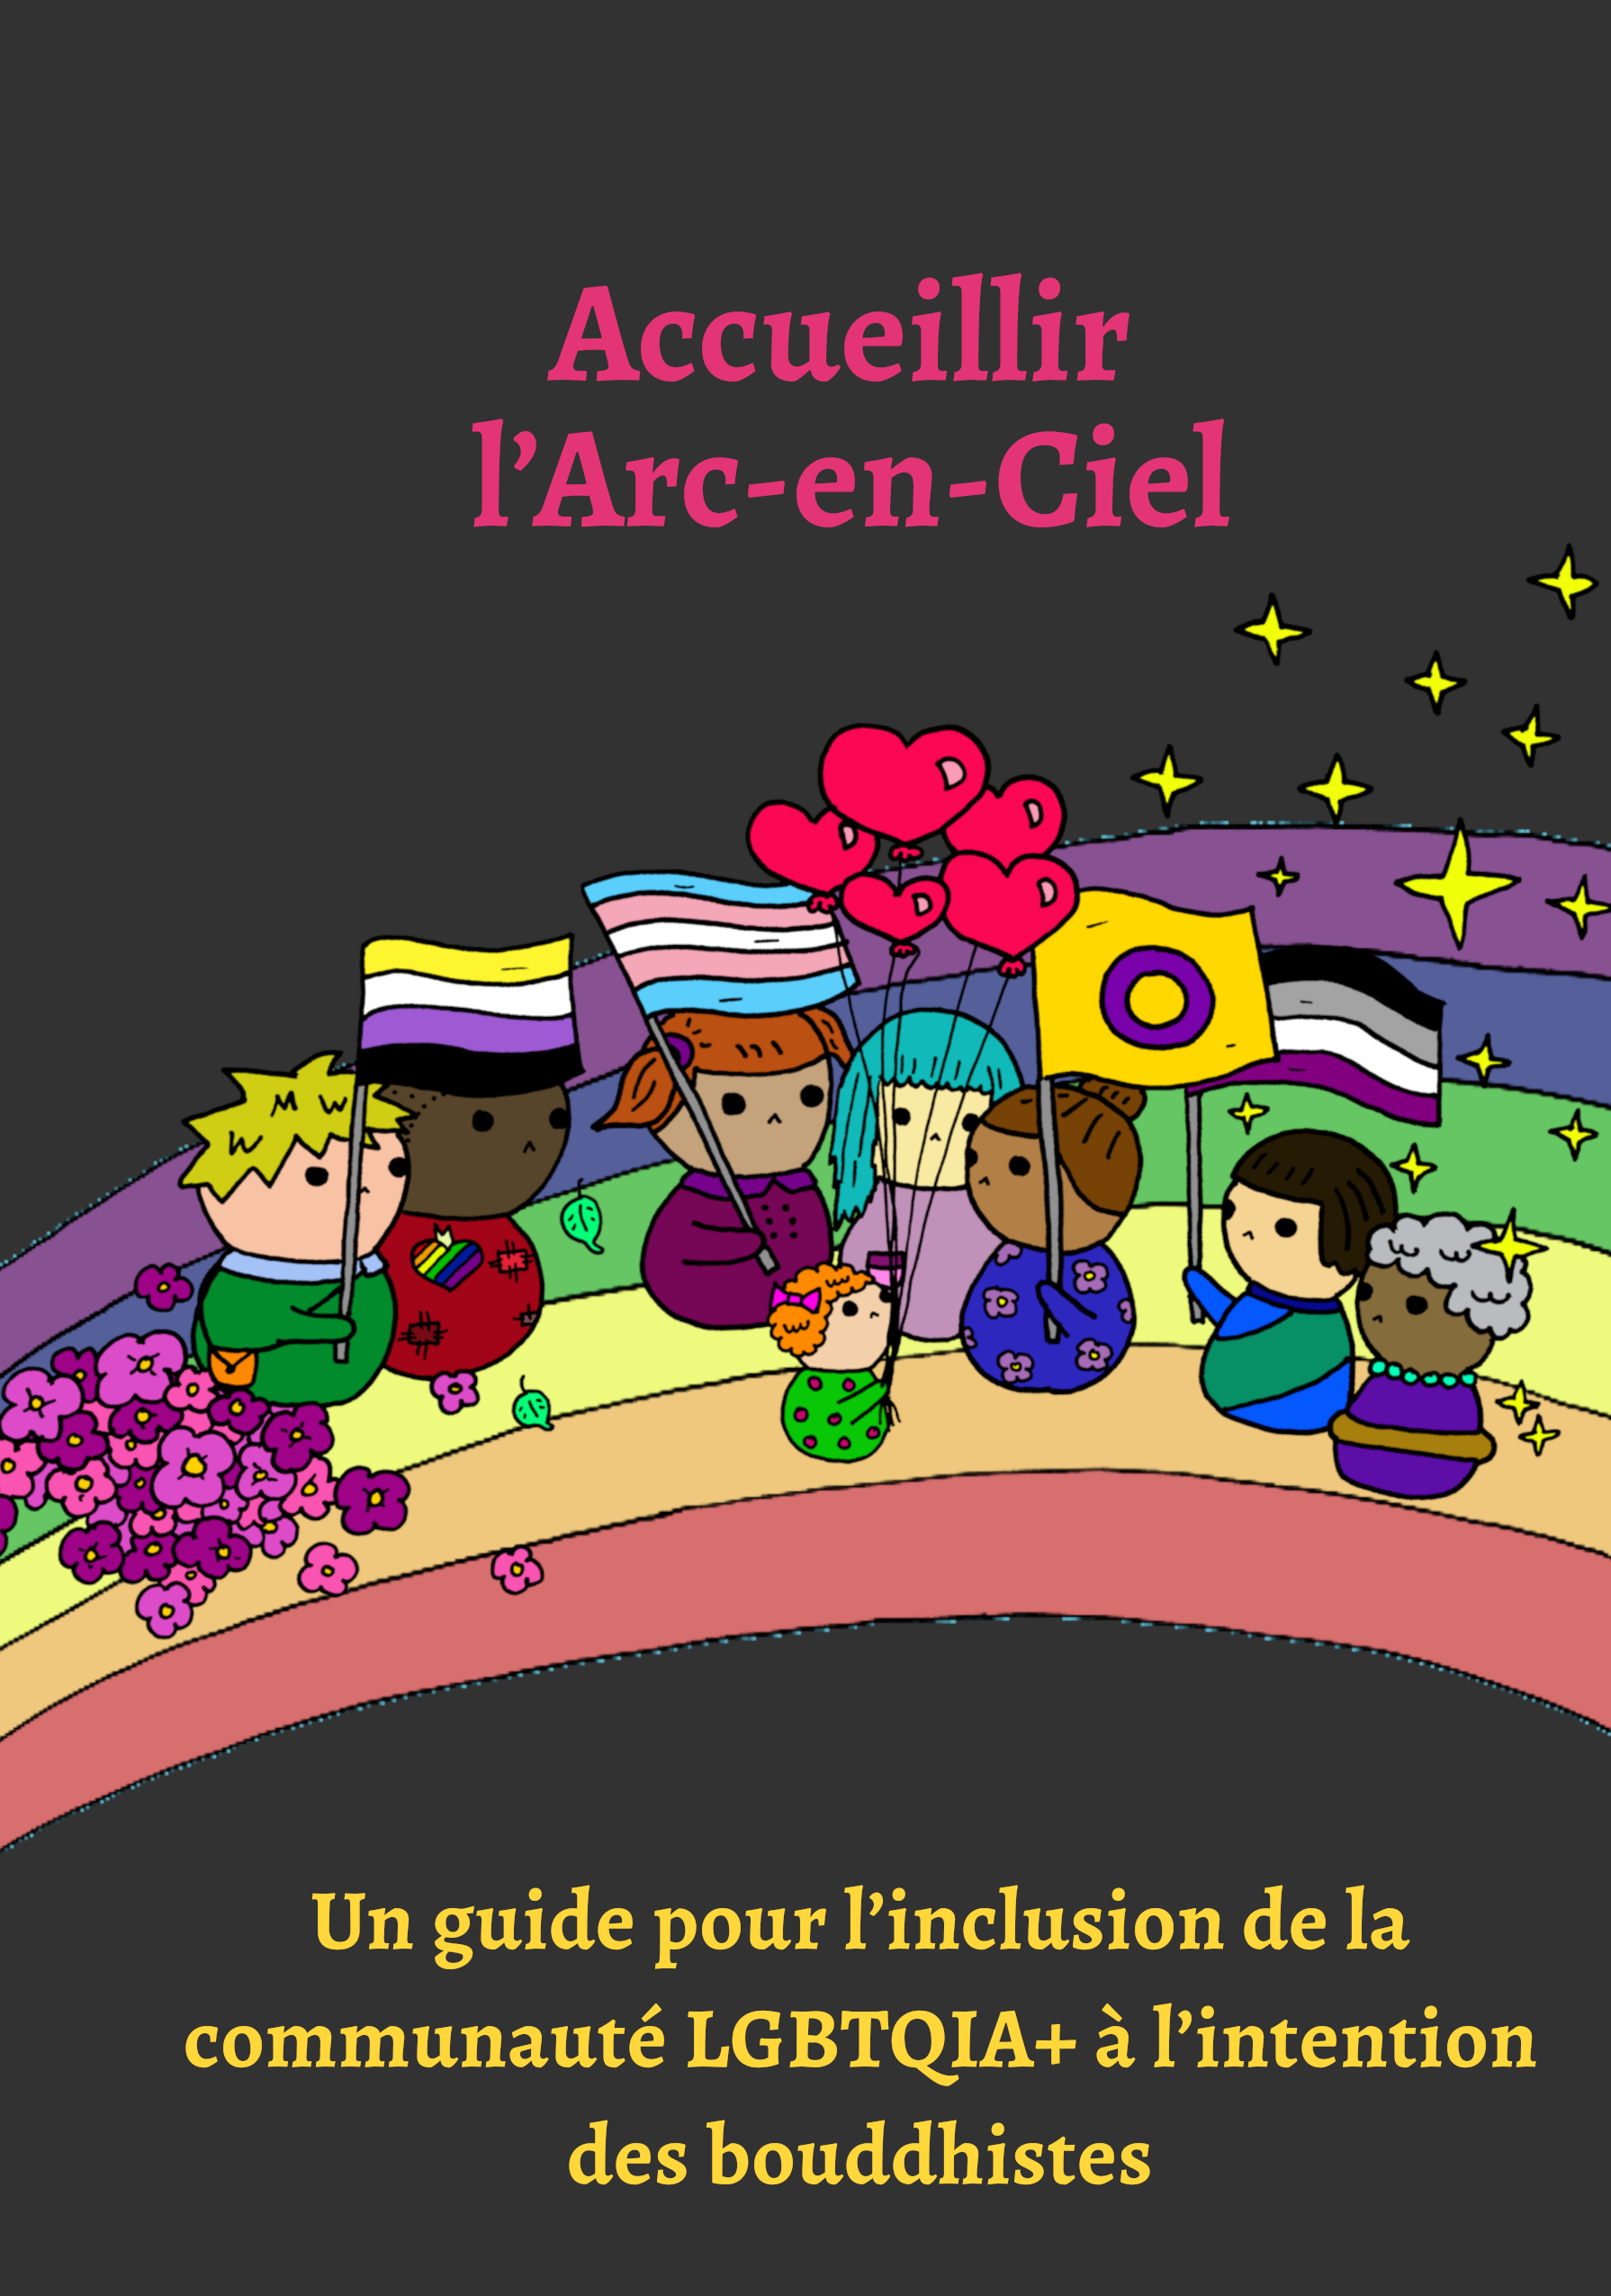
\includegraphics[width=\paperwidth]{front_francais}}
\end{figure}

\restoregeometry

\begin{figure}[h]
    \makebox[150pt]{%
    
\includegraphics[width=0.4\paperwidth]{1bw.png}}
\end{figure}

\begin{center}

\thispagestyle{empty}

\sffamily

\caps{\Huge \textbf{Accueillir l’Arc-en-Ciel}}

\medskip

\textit{ }

\caps{\LARGE \textbf{Un guide pour l’inclusion de la communauté \mbox{LGBTQIA+} à l’intention des bouddhistes}}

\end{center}

\begin{figure}[h]
    \makebox[450pt]{%
    
\includegraphics[width=0.4\paperwidth]{1bw2.png}}
\end{figure}

\newpage
\thispagestyle{empty}
\mbox

\newpage
\thispagestyle{empty}
\mbox

\tableofcontents
\thispagestyle{empty}
\markboth{}{}

\bigskip{}

\begin{figure}[h]
    \makebox[150pt]{%
    
\includegraphics[width=0.4\paperwidth]{2bw.png}}
\end{figure}

\newpage
\thispagestyle{empty}

\rmfamily

\begin{center}\end{center}
\begin{center}

\vfill
\color{gray}
\caps{\LARGE \textit{\textbf{Puissent tous les êtres être heureux.}}}

\vfill

\end{center}

\begin{figure}[h]
    \centering
    \makebox[0pt]{%
    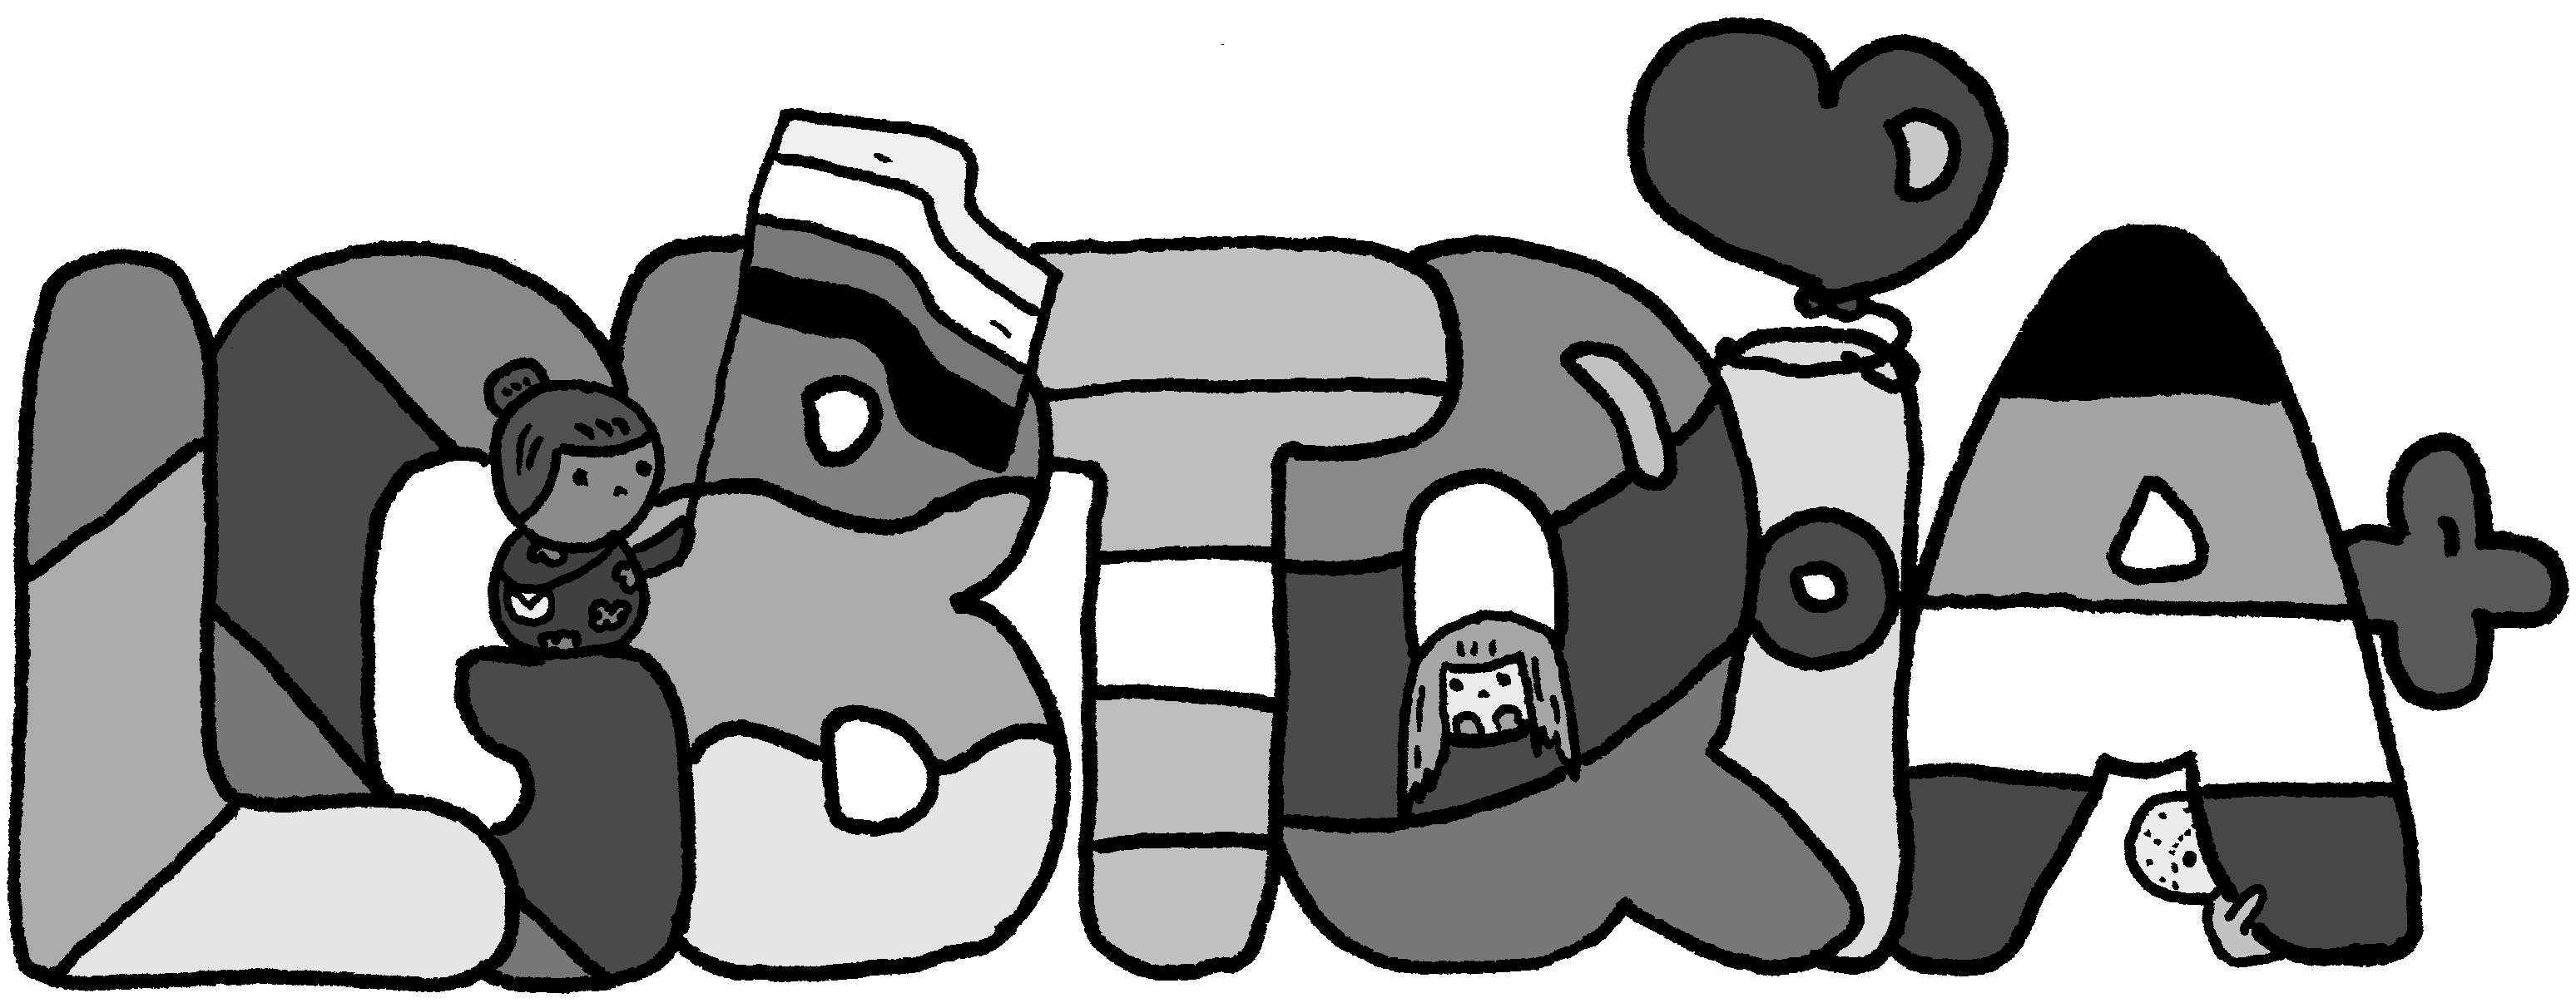
\includegraphics[width=0.8\paperwidth]{2-3bw.png}}
\end{figure}

\thispagestyle{empty}

\begin{figure}[h]
    \makebox[450pt]{%
    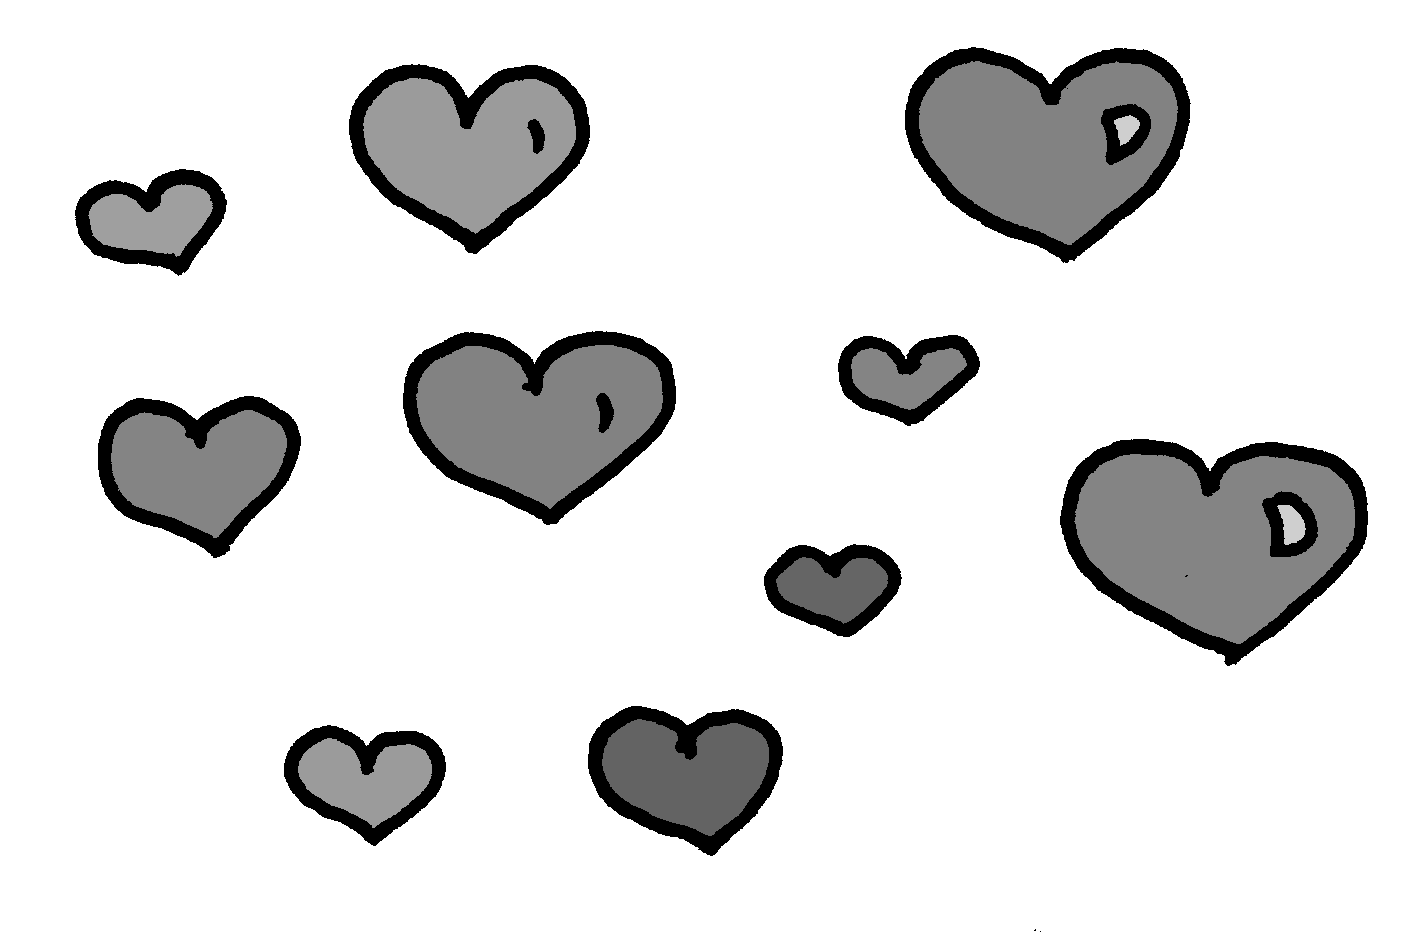
\includegraphics[width=0.4\paperwidth]{2bw2.png}}
\end{figure}

\thispagestyle{empty}

\mainmatter
\newpage
\thispagestyle{empty}
\color{darkgray}
\begingroup
\begin{quote}
\doublespacing
\centering
\textit{\Large \textbf{Tant que des individus ou des organisations bouddhistes se rendent coupables d'homophobie, de biphobie, de transphobie ou d'interphobie, ils perpétuent la haine, la violence et les abus.}}
\end{quote}
\endgroup

\medskip

\begin{figure}[h]
    \centering
    \makebox[0pt]{%
    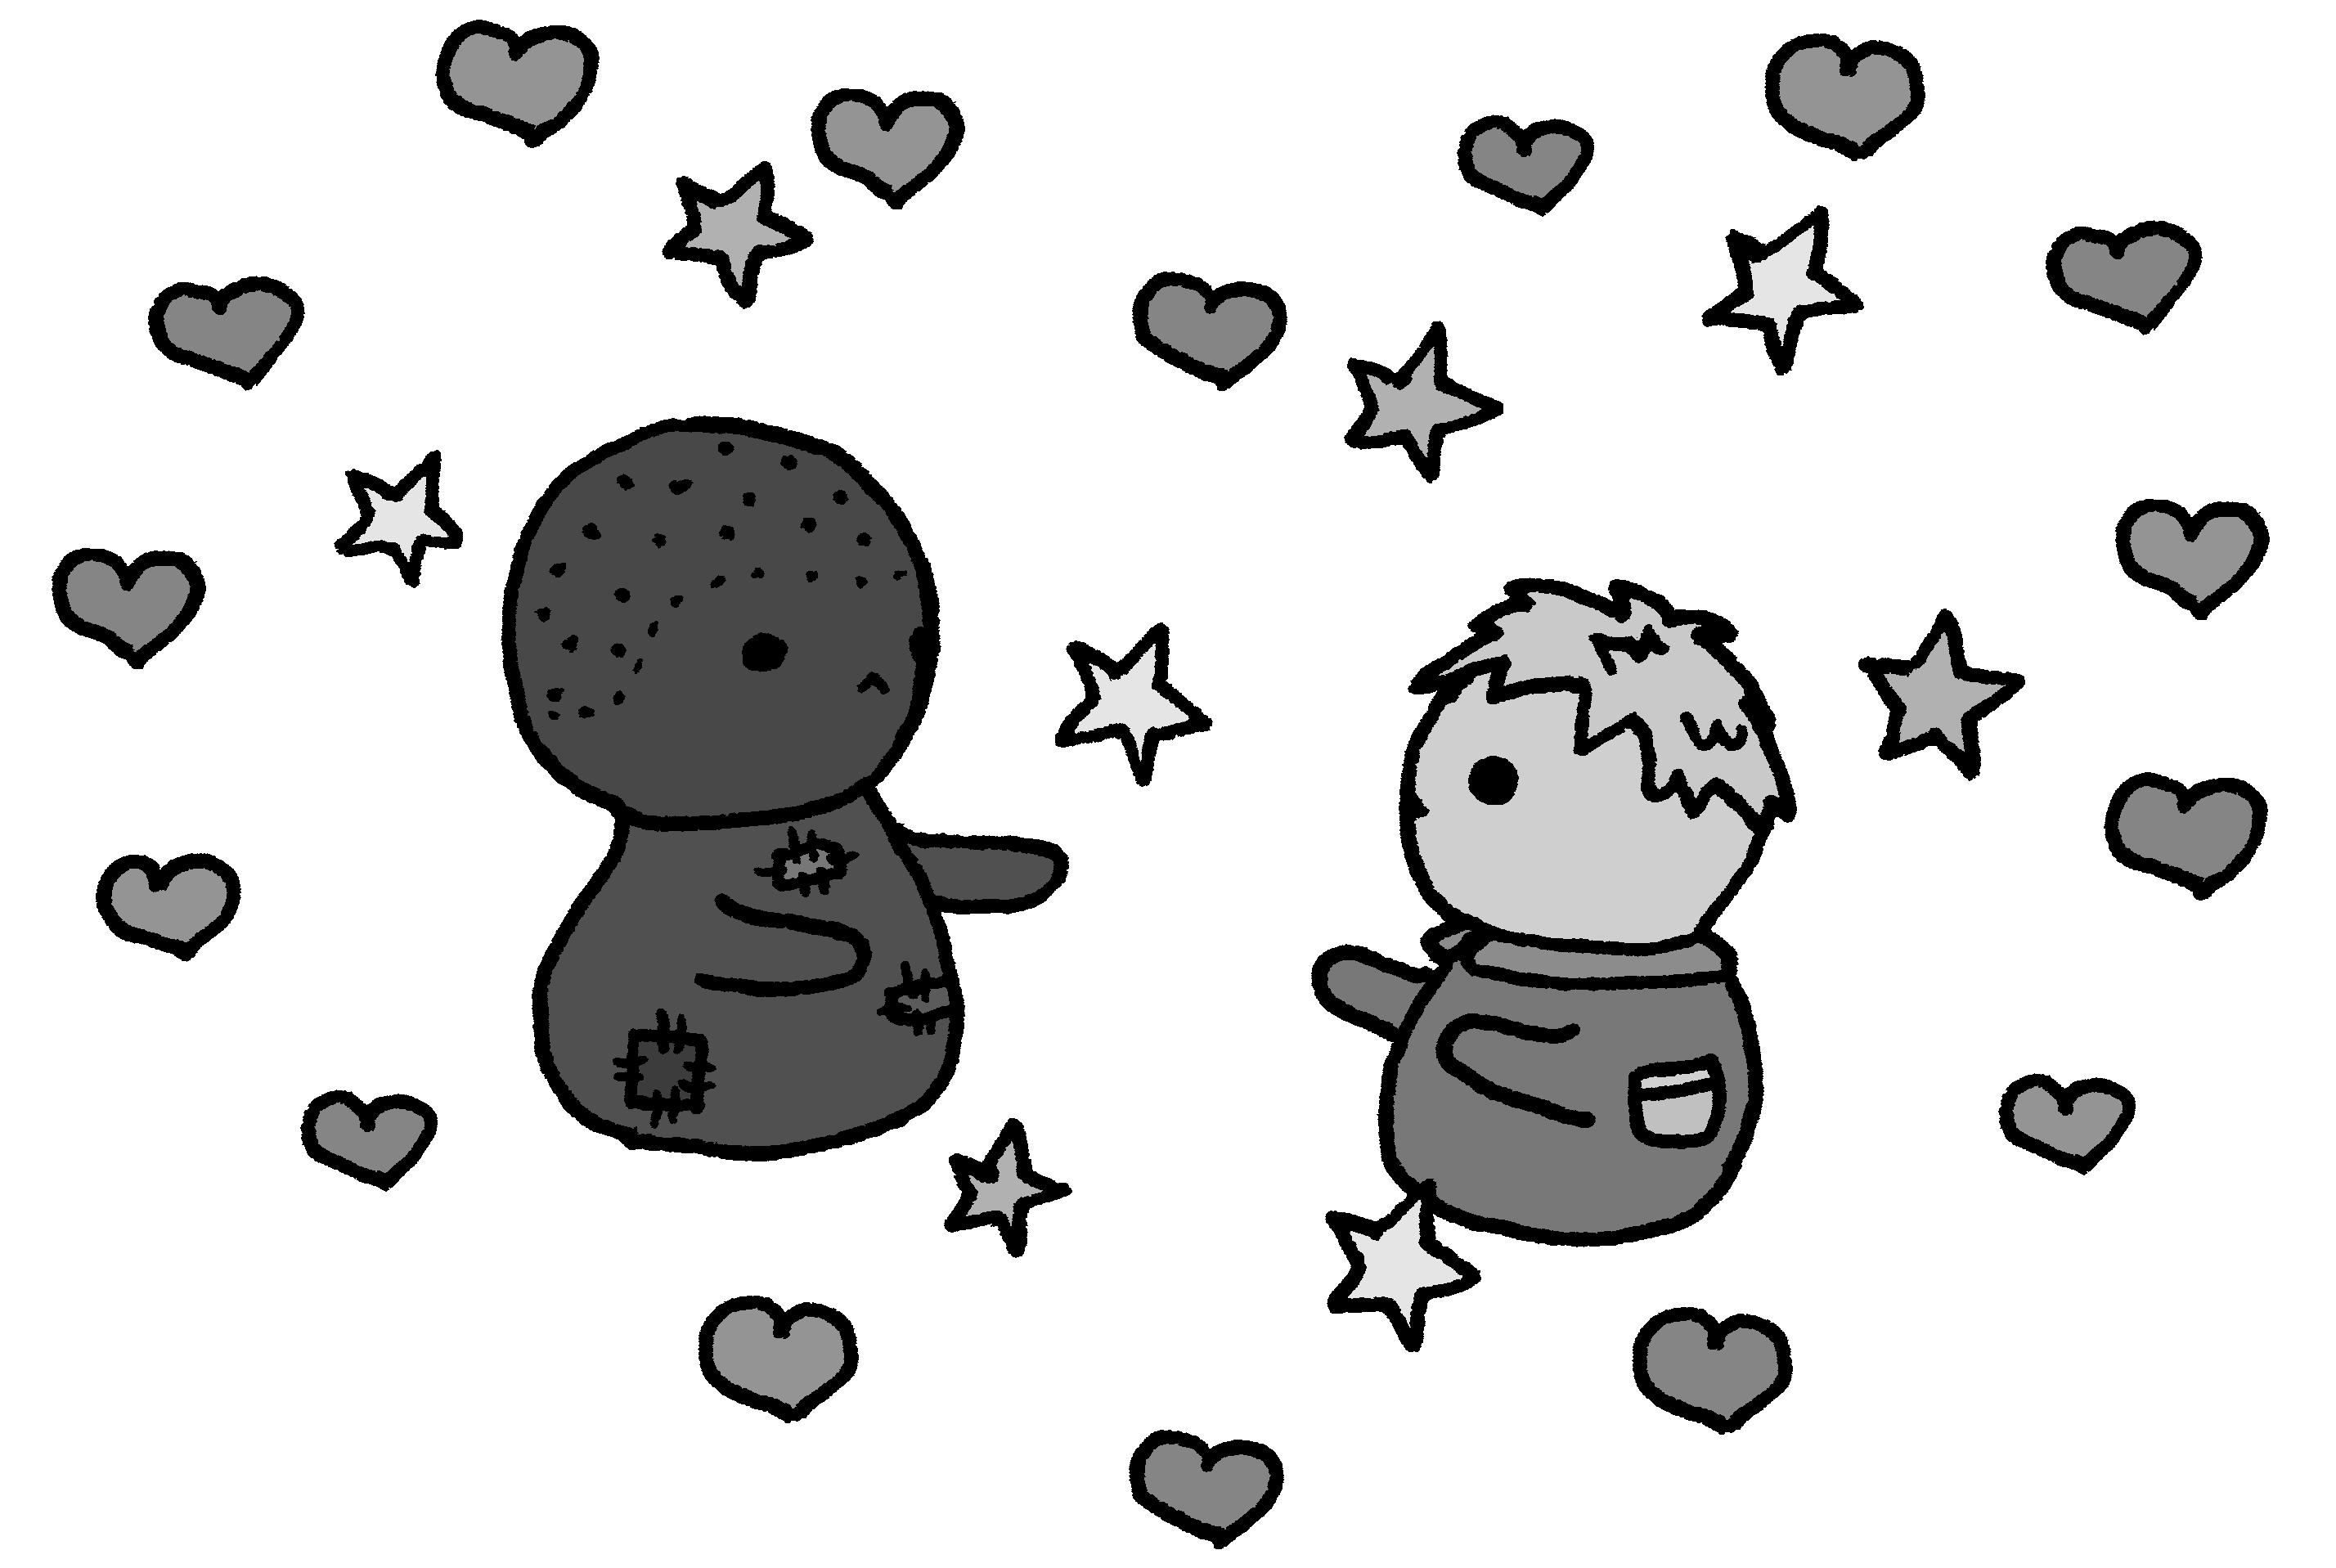
\includegraphics[width=0.8\paperwidth]{6-7bw.png}}
\end{figure}

\begingroup
\begin{quote}
\centering
\doublespacing
\textit{\Large \textbf{Si nous comprenons mieux comment il est possible d'améliorer l'accueil et l'inclusion des personnes \mbox{LGBTQIA+}, nous pouvons vraiment pratiquer l'amour bienveillant et la compassion à l'égard de tous les membres de nos communautés.}}
\end{quote}
\endgroup
\color{black}

\setlength{\parindent}{15pt}
\chapter*{Accueillir l’Arc-en-ciel}
\addcontentsline{toc}{chapter}{Accueillir l’Arc-en-ciel}
\markboth{Accueillir l’Arc-en-ciel}{Accueillir l’Arc-en-ciel}

\begin{wrapfigure}{hl}{0.25\textwidth}
    \makebox[150pt]{%
    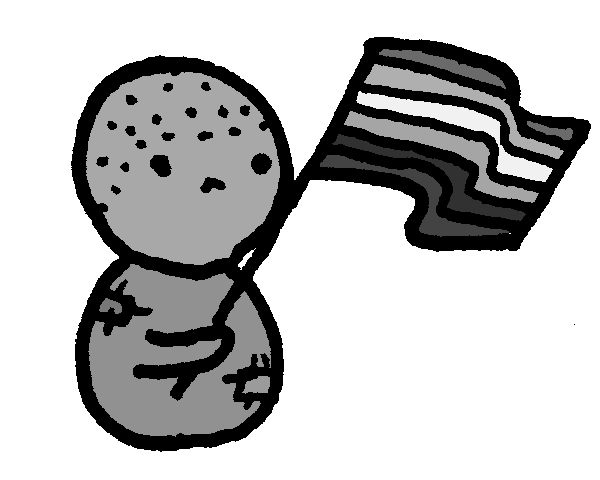
\includegraphics[width=0.25\textwidth]{2bw3.png}}
\end{wrapfigure}
\noindent La communauté bouddhiste \mbox{LGBTQIA+} Rainbodhi a rassemblé dans ce livret quelques conseils pratiques pour contribuer à faire des temples, monastères et organisations bouddhistes des lieux sûrs et accueillants pour les bouddhistes \mbox{LGBTQIA+}.

\smallskip

\begingroup
\begin{quote}
\centering
\doublespacing
\textit{\large \textbf{\textcolor{darkgray}{Ensemble, nous pouvons faire en sorte que nos centres bouddhistes soient des espaces plus sécurisants et plus inclusifs pour notre communauté arc-en-ciel.}}}
\end{quote}
\endgroup

\phantomsection
\section*{Le sigle arc-en-ciel}
\addcontentsline{toc}{section}{Le sigle arc-en-ciel}

\noindent L’abréviation \mbox{« \mbox{LGBTQIA+} »} signifie lesbienne, gay, bisexuel, transgenre, queer, intersexe et asexuel. Le signe \mbox{« + »} indique que d’autres identités sont possibles. Nous appelons cette abréviation le \mbox{« s}igle arc-en-cie\mbox{l »}, parce que notre communauté est constituée de nombreux groupes différents, comme les couleurs qui composent l’arc-en-ciel.

Le sigle \mbox{LGBTQIA+} couvre un large éventail d’identités, qui se rapportent notamment à des caractéristiques physiques, à l’orientation sexuelle des personnes et à leurs identités de genre. Ces groupes sont assez différents les uns des autres, mais ils se recoupent parfois.
Ainsi, les termes \mbox{« lesbienne »}, \mbox{« gay »} et \mbox{« bisexuel.le »} font référence à l’orientation sexuelle ; \mbox{« transgenre »} renvoie à l’identité de genre ; \mbox{« queer »} peut avoir trait à l’identité de genre ou à la sexualité ; \mbox{« intersexe »} désigne les personnes nées avec des caractéristiques physiques à la fois féminines et masculines, et \mbox{« asexuel.le »} se réfère à une absence de sexualité. Des combinaisons de ces différentes facettes sont également possibles.

Bien que les identités \mbox{LGBTQIA+} soient différentes, ces groupes font tous face à des défis communs, et notamment à des préjugés, à la discrimination, à des obstacles juridiques et à la violence, juste parce qu’ils sont qui ils sont.

\phantomsection
\section*{Créer le changement ensemble}
\addcontentsline{toc}{section}{Créer le changement ensemble}

\noindent Les personnes \mbox{LGBTQIA+} sont souvent confrontées au rejet et à l’oppression au sein de la société et des communautés religieuses. Le Bouddha s’est souvent prononcé contre la discrimination, affirmant que tous les êtres vivants méritaient d’êtres aimés sans distinction.
Tout le monde étant à même d’atteindre l’éveil, nous devons nous assurer de n’exclure personne de nos communautés bouddhistes.

Nous ne sommes pas toujours conscients que nos organisations bouddhistes, nos temples et nos centres de retraite ne sont pas forcément des lieux accueillants pour la communauté \mbox{LGBTQIA+}. Les personnes peuvent ne pas se rendre compte que leurs actions et leurs paroles sont susceptibles de porter préjudice aux personnes \mbox{LGBTQIA+}. Les organisations peuvent ne pas voir qu’elles excluent les personnes \mbox{LGBTQIA+}, ni comment.

La bonne nouvelle, c’est que les choses sont en train de changer, et nous pouvons faire partie de ce changement.

\phantomsection
\section*{Être à l’écoute de notre communauté}
\addcontentsline{toc}{section}{Être à l’écoute de notre communauté}

\noindent Il est essentiel d’écouter la voix des bouddhistes \mbox{LGBTQIA+} pour comprendre leurs expériences. Une étude récente, parrainée par Rainbodhi et menée par le Dr Stephen Kerry de l’Université Charles Darwin, a révélé que les communautés bouddhistes australiennes peuvent être des environnements difficiles pour les bouddhistes \mbox{LGBTQIA+}1. S’agissant de leurs propres centres bouddhistes, les personnes interrogées ont rapporté les faits suivants:

\begin{itemize}[label=\textbullet, leftmargin=*]
\setlength\itemsep{-0.3em}
  \item 61\% ont eu le sentiment que les centres bouddhistes ignoraient les personnes \mbox{LGBTQIA+}, les réduisaient au silence ou fermaient les yeux sur leurs problèmes
  \item 55\% ont parfois été réticent.es à divulguer leur identité \mbox{LGBTQIA+}
  \item 54\% ont été victimes ou témoins d’actes ou de propos sexistes
  \item 37\% ont été victimes ou témoins d’actes ou de propos homophobes
  \item 26\% ont été victimes ou témoins d’actes ou de propos transphobes ou ont vu/entendu des personnes être mégenrées
  \item 26\% ont été victimes ou témoins d’actes ou de propos racistes
  \item 16\% se sont entendu dire que leur identité \mbox{LGBTQIA+} était incompatible avec les enseignements bouddhistes.
\end{itemize}

\begin{wrapfigure}{l}{0.15\textwidth}
    \centering
    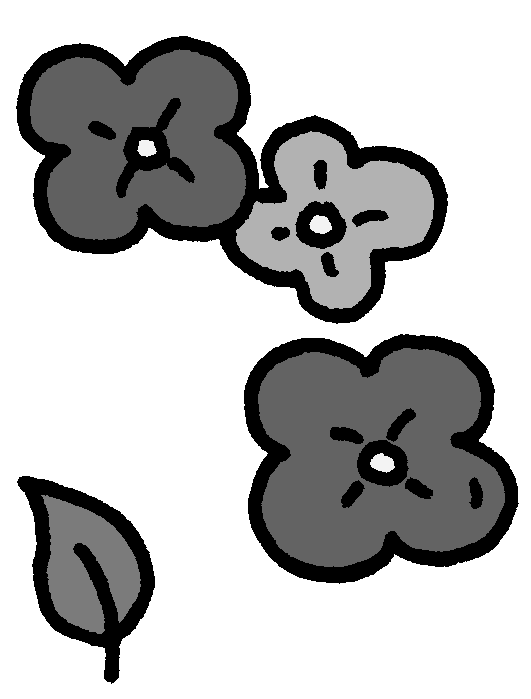
\includegraphics[width=0.15\textwidth]{2bw4.png}
\end{wrapfigure}

Ces résultats montrent que les centres bouddhistes ne sont pas toujours des espaces sûrs pour les bouddhistes \mbox{LGBTQIA+}. Reconnaître l’existence de préjugés et de discriminations est une première étape importante pour apporter les changements nécessaires afin de créer des communautés bouddhistes plus sécurisantes et plus inclusives.

\phantomsection
\section*{Le bouddhisme a un passé (et un avenir) \mbox{LGBTQIA+}}
\addcontentsline{toc}{section}{Le bouddhisme a un passé (et un avenir) \mbox{LGBTQIA+}}

\noindent Il y a toujours eu des personnes homosexuelles, trans et intersexes dans l’histoire de l’humanité. Les personnes \mbox{LGBTQIA+} sont aussi des personnes spirituelles, il n’est donc pas surprenant de constater que le bouddhisme entretient des relations de longue date avec la communauté \mbox{LGBTQIA+}.

Des textes bouddhistes anciens traitent de l’attirance pour le même sexe et de la sexualité sans aucun jugement moral ni négativité. Il existe également des récits de laïcs/laïques et de moines/moniales qui ont changé de genre. La société indienne ancienne reconnaissait une catégorie de personnes qui n’étaient considérées ni comme des hommes ni comme des femmes, que nous pourrions appeler transgenres ou troisième genre aujourd’hui, et une autre catégorie de personnes qui avaient à la fois des caractéristiques sexuelles masculines et féminines, que nous désignerions peut-être aujourd’hui par le terme \mbox{« intersexes »}. Certains de ces groupes ont été stigmatisés et mis au ban de la société tout au long de l’histoire du bouddhisme, et pour certains d’entre eux, cette discrimination se poursuit aujourd’hui.

\subsubsection*{Les Fiertés dans le bouddhisme}

\noindent Des personnes \mbox{LGBTQIA+} ont contribué à l’épanouissement du bouddhisme en tant que moines/moniales, fidèles laïques, enseignant.es et chercheurs.euses universitaires.
Cependant, leurs histoires sont souvent oubliées, ou leurs expériences passées sous silence.
À l’heure où la société commence à mieux comprendre et accepter les personnes LGBTQIA + en général, le moment est venu pour les pratiquant.es et organisations bouddhistes de célébrer notre communauté arc-en-ciel et de lui montrer leur soutien de manière concrète.
Les personnes \mbox{LGBTQIA+} pourront ainsi être sûres d’être considérées comme des membres à part entière de la communauté bouddhiste.

\begingroup
\begin{figure}[h]
    \centering
    \makebox[0pt]{%
    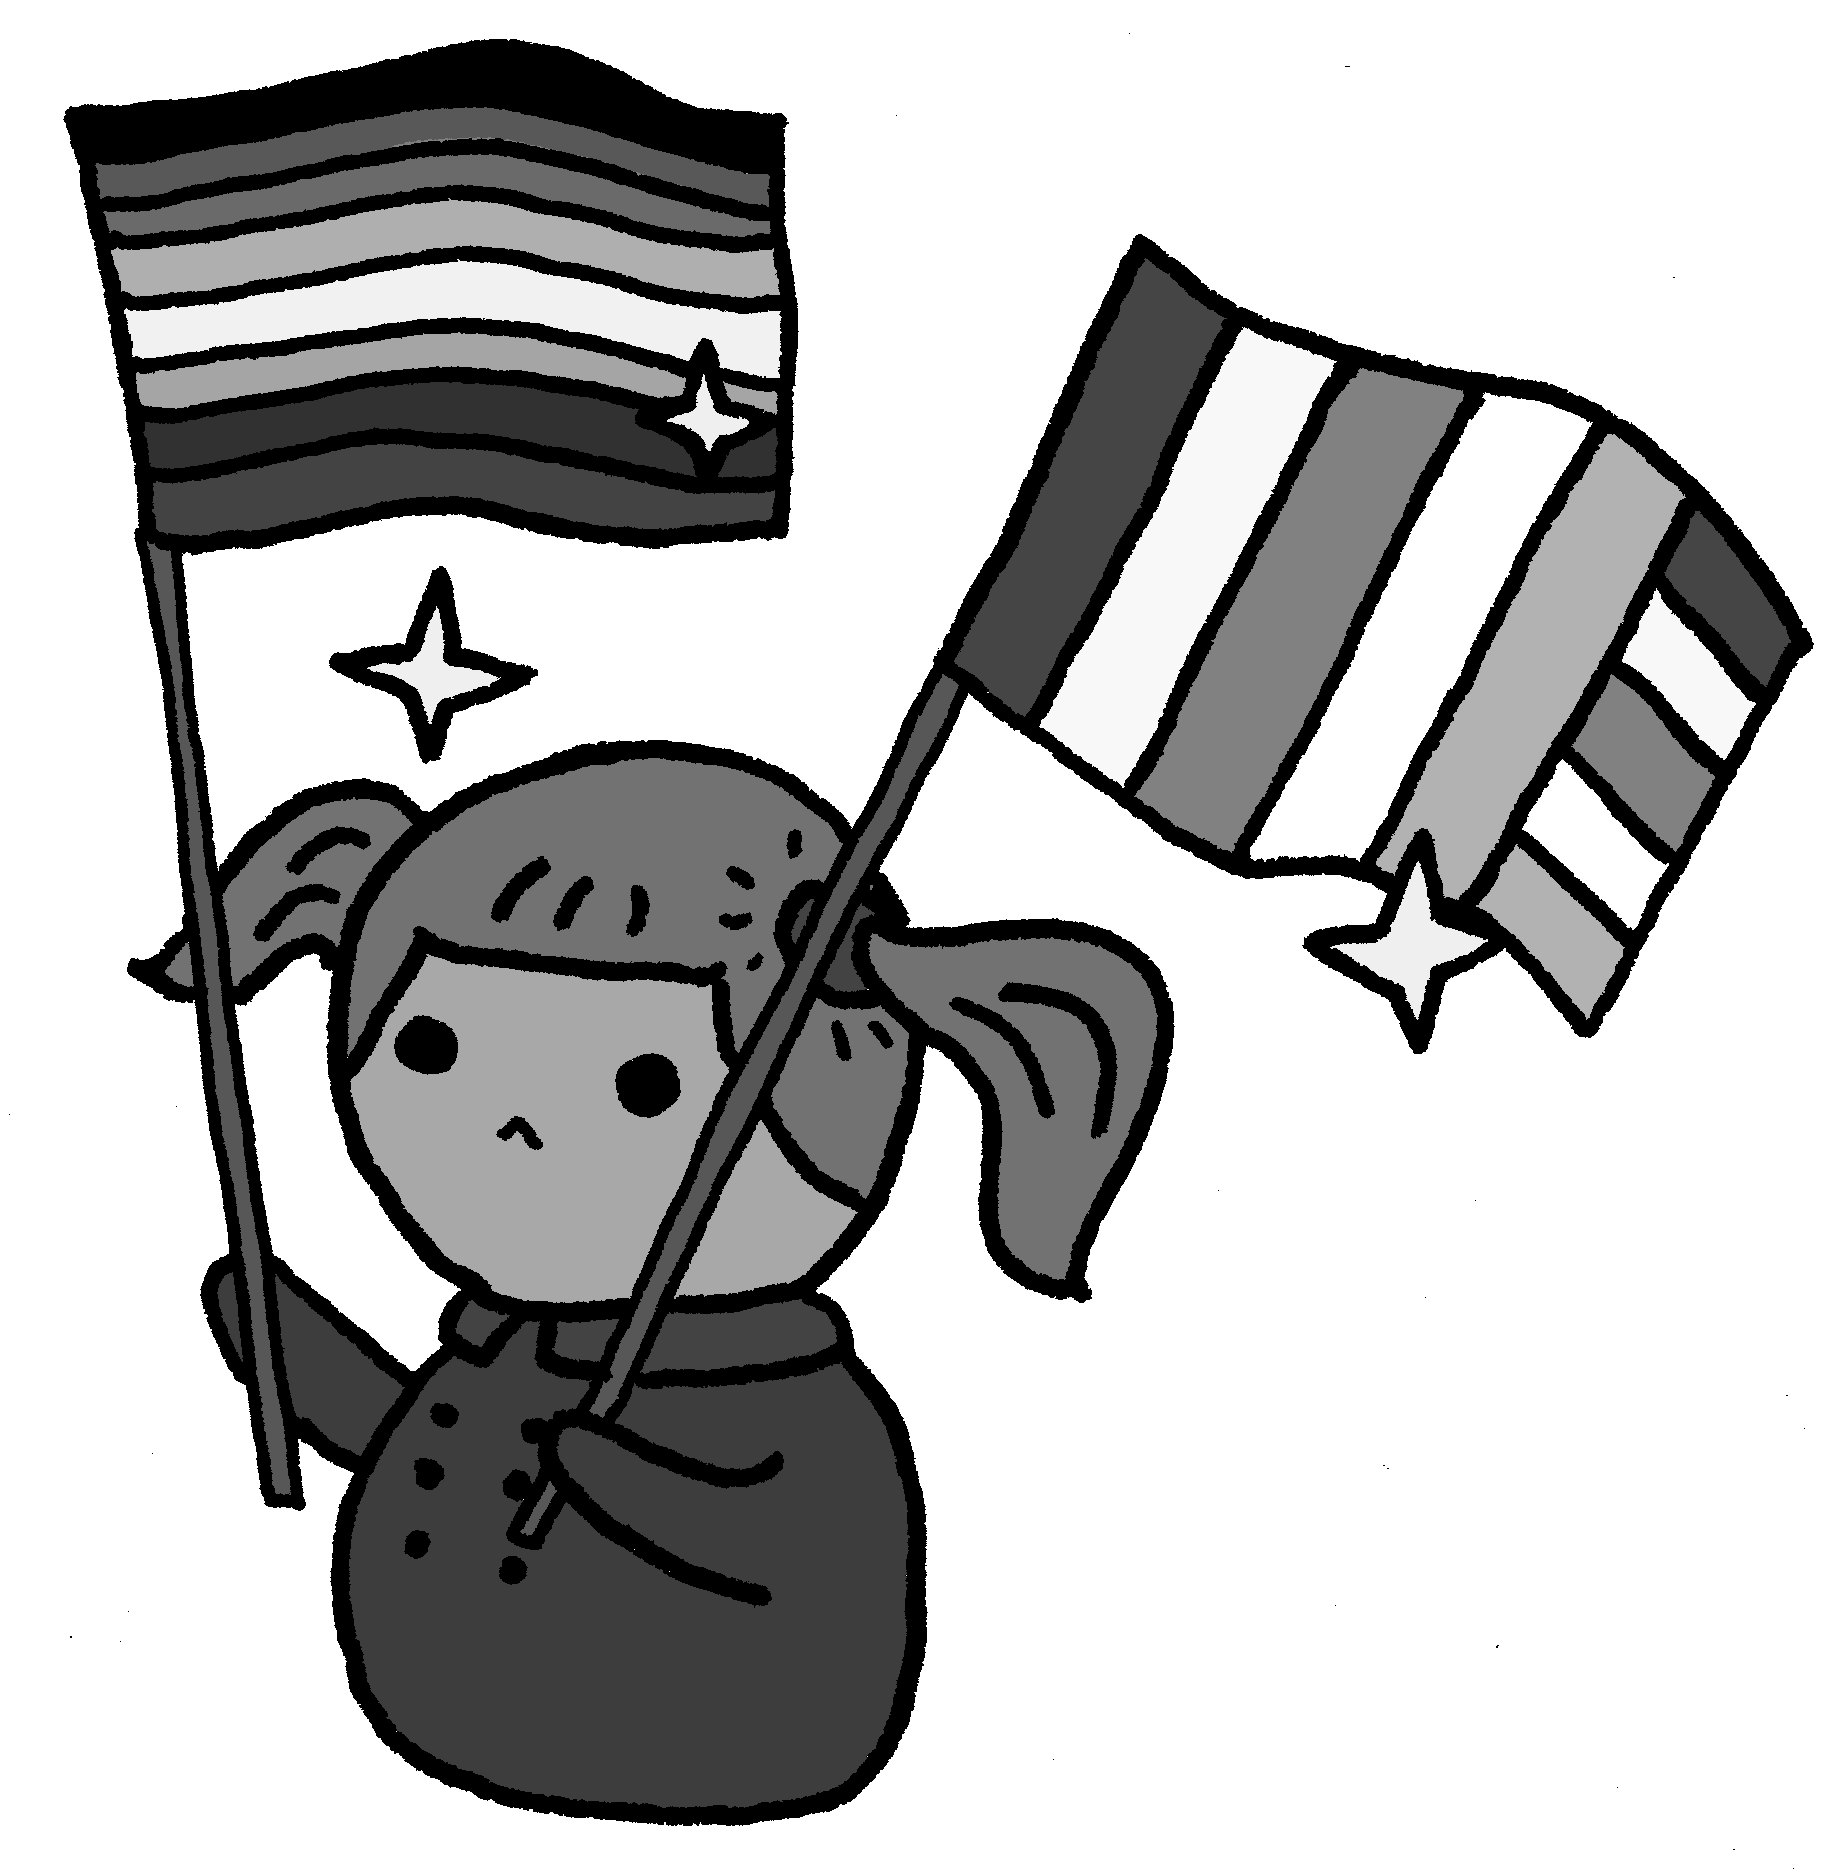
\includegraphics[width=0.21\paperwidth]{9bw.png}}
\end{figure}

\begin{quote}
\centering
\doublespacing
\textit{\Large \textbf{\textcolor{darkgray}{Chaque personne, quels que soient son genre et sa sexualité, doit pouvoir vivre sa vie sans craindre d’être rejetée, et être fière de qui elle est.}}}
\end{quote}
\endgroup

\chapter*{Soyez un.e ami.e spirituel.le pour les bouddhistes \mbox{LGBTQIA+}}
\addcontentsline{toc}{chapter}{Soyez un.e ami.e spirituel.le pour les bouddhistes \mbox{LGBTQIA+}}
\markboth{Accueillir l’Arc-en-ciel}{Soyez un.e ami.e spirituel.le pour les bouddhistes \mbox{LGBTQIA+}}

\begingroup
\begin{quote}
\centering
\textit{\Large \textbf{\textcolor{darkgray}{\mbox{Les ami.es de bien sont la voie spirituelle complète.}}}}
\end{quote}
\endgroup

\phantomsection
\section*{Être un.e allié.e}
\addcontentsline{toc}{section}{Être un.e allié.e}

\noindent Être un.e ami.e spirituel.le pour autrui est un aspect fondamental du bouddhisme. Vous pouvez aider d’autres personnes à se sentir en sécurité et bienvenues en portant leurs voix, en étant un.e allié.e pour la communauté \mbox{LGBTQIA+}.

Un.e allié.e est quelqu’un qui soutient les droits civils des personnes \mbox{LGBTQIA+} et combat activement l'homophobie, la biphobie, la transphobie et l'interphobie. Les allié.es sont souvent des personnes hétérosexuelles et/ou cisgenres (à savoir des personnes qui s’identifient au sexe qui leur a été assigné à la naissance). Les allié.es reconnaissent qu’iels ont le privilège de ne pas subir les mêmes désavantages sociaux que les personnes LGBTQIA + et utilisent cette position de privilège pour combattre la discrimination qui s’exerce à l’encontre de ces communautés.

Un.e allié.e peut aussi être quelqu’un qui fait partie de la communauté LGBTQIA + et soutient un groupe auquel iel ne s’identifie pas. Par exemple, un homme homosexuel cisgenre peut être un allié pour les personnes transgenres, ou une personne intersexe peut soutenir les droits des personnes attirées par le même sexe.

Les allié.es aident les personnes \mbox{LGBTQIA+} à expliquer les problèmes qu’elles rencontrent dans le monde. Pour être un.e bon.ne allié.e, il est d’abord important d’écouter les personnes \mbox{LGBTQIA+} et de se renseigner sur leurs expériences diverses. Cela suppose, par exemple, de connaître des choses élémentaires, comme la signification des lettres de l’acronyme arc-en-ciel, la différence entre sexualité et genre, en quoi les problèmes qui affectent les personnes transgenres sont différents de ceux qui touchent les personnes LGB, ou les droits fondamentaux pour lesquels se battent les personnes intersexes. N’importe qui peut être un.e allié.e indépendamment de sa sexualité ou de son genre.
\begin{wrapfigure}{hr}{0.25\textwidth}
    \centering
    
\includegraphics[width=0.25\textwidth]{12bw.png}
\end{wrapfigure}

\begin{quote}
\textit{\large \textbf{\textcolor{darkgray}{Être un.e allié.e est un acte d’amitié et de compassion.}}}
\end{quote}

\phantomsection
\section*{Promouvoir l’inclusion}
\addcontentsline{toc}{section}{Promouvoir l’inclusion}

\noindent Il est bon de rappeler qu’il y a déjà des personnes \mbox{LGBTQIA+} dans les communautés bouddhistes. Nous ne devrions jamais partir du principe que tout le monde est hétérosexuel ou qu’il est possible de déterminer d’un simple regard le genre d’une personne ou les pronoms que celle-ci souhaite que l’on emploie à son égard. Tenir compte du fait que des personnes \mbox{LGBTQIA+} fréquentent les temples, les retraites et les centres est la première étape pour devenir plus inclusif.

Souvent, les personnes \mbox{LGBTQIA+} se sentent invisibilisées dans les communautés bouddhistes, et leurs besoins spécifiques ne sont pas reconnus ni pris en compte. Parfois, elles ne peuvent pas s’ouvrir sur leur identité parce qu’elles craignent d’être rejetées et peuvent être mal à l’aise à l’idée de parler des problèmes qui les concernent. Elles peuvent douter que les communautés bouddhistes soient un espace sûr, à la suite d’une mauvaise expérience passée dans un autre centre bouddhiste ou avec la religion en général. Faire savoir aux bouddhistes \mbox{LGBTQIA+} qu’iels sont les bienvenu.es dans nos communautés, c’est faire preuve de bienveillance et d’amitié spirituelle. L’inclusion consiste à faire savoir aux bouddhistes arc-en-ciel qu’iels sont considéré.es comme des membres à part entière de la communauté et sont apprécié.es.

\subsubsection*{L’inclusion est synonyme de changements}

\noindent Accueillir des personnes \mbox{LGBTQIA+} dans votre communauté est un bon début, mais pour véritablement les inclure, il vous faudra aussi veiller à éliminer les barrières qui les excluent actuellement. Pour ce faire, il est essentiel de comprendre le point de vue des personnes \mbox{LGBTQIA+}, de prendre conscience des choses qui leur causent du tort et d’apporter les changements nécessaires pour les éviter. Cela peut nécessiter de modifier les pratiques administratives, et par exemple de remanier les formulaires d’adhésion et d’inscription ne proposant que des options \mbox{« homme »} ou \mbox{« femme »}. Ou de revoir la dispositions des lieux, par exemple en prévoyant des toilettes non genrées et des possibilités d’hébergement mixtes. Cela peut aussi supposer un changement au niveau personnel, et par exemple une plus grande attention aux mots que nous employons ou aux types de questions que nous posons afin de ne pas donner aux personnes \mbox{LGBTQIA+} le sentiment qu’elles ne sont pas à leur place.

Les centres bouddhistes devraient mettre en place des politiques d’inclusion afin que toute personne sache qu’elle est la bienvenue. Une charte publique prévoyant des procédures ad hoc est nécessaire pour appuyer ces politiques d’inclusion. Celle-ci doit garantir que toute personne accueillie dans un espace puisse s’y sentir en sécurité pendant son séjour et sache qu’elle dispose de voies de recours en cas de problème.

\phantomsection
\section*{Célébrer la diversité} 
\addcontentsline{toc}{section}{Célébrer la diversité}

\noindent Il existe de nombreuses façons pour les bouddhistes et leurs organisations de montrer leur soutien à la communauté arc-en-ciel. Célébrer la diversité offre de nombreuses occasions de voir éclore la joie empathique face au bonheur d’autrui.

\begin{itemize}[label=\textbullet, leftmargin=*]
  \setlength\itemsep{-0.3em}
  \item Inscrivez-vous à une formation sur la diversité et l’inclusion \mbox{LGBTQIA+} pour vous-même et pour l’ensemble de votre organisation. Encouragez d’autres organisations bouddhistes à faire de même.
  \item Utilisez des affiches ou des autocollants pour faire savoir à votre communauté que vous soutenez l’inclusion des personnes \mbox{LGBTQIA+} dans votre centre et ajoutez un symbole arc-en-ciel \mbox{« e}space sû\mbox{r »} sur votre site web et vos supports publicitaires.
  \item Mentionnez que votre organisation accueille et soutient les personnes \mbox{LGBTQIA+} lors de conférences et d’événements.
  \item Organisez un événement Pride pour les personnes \mbox{LGBTQIA+} et leurs alliés au sein de votre communauté.
  \item Invitez les personnes \mbox{LGBTQIA+} à participer à tous les aspects de votre organisation, y compris l’enseignement, l’administration et le bénévolat.
  \item Mettez en place des procédures accessibles au public permettant de soulever des questions, problèmes ou préoccupations en matière de discriminations ou de préjugés et de s’assurer qu’il y aura bel et bien un suivi et que les difficultés rencontrées seront résolues.
\end{itemize}

\begin{figure}[h]
    \centering
    \makebox[0pt]{%
    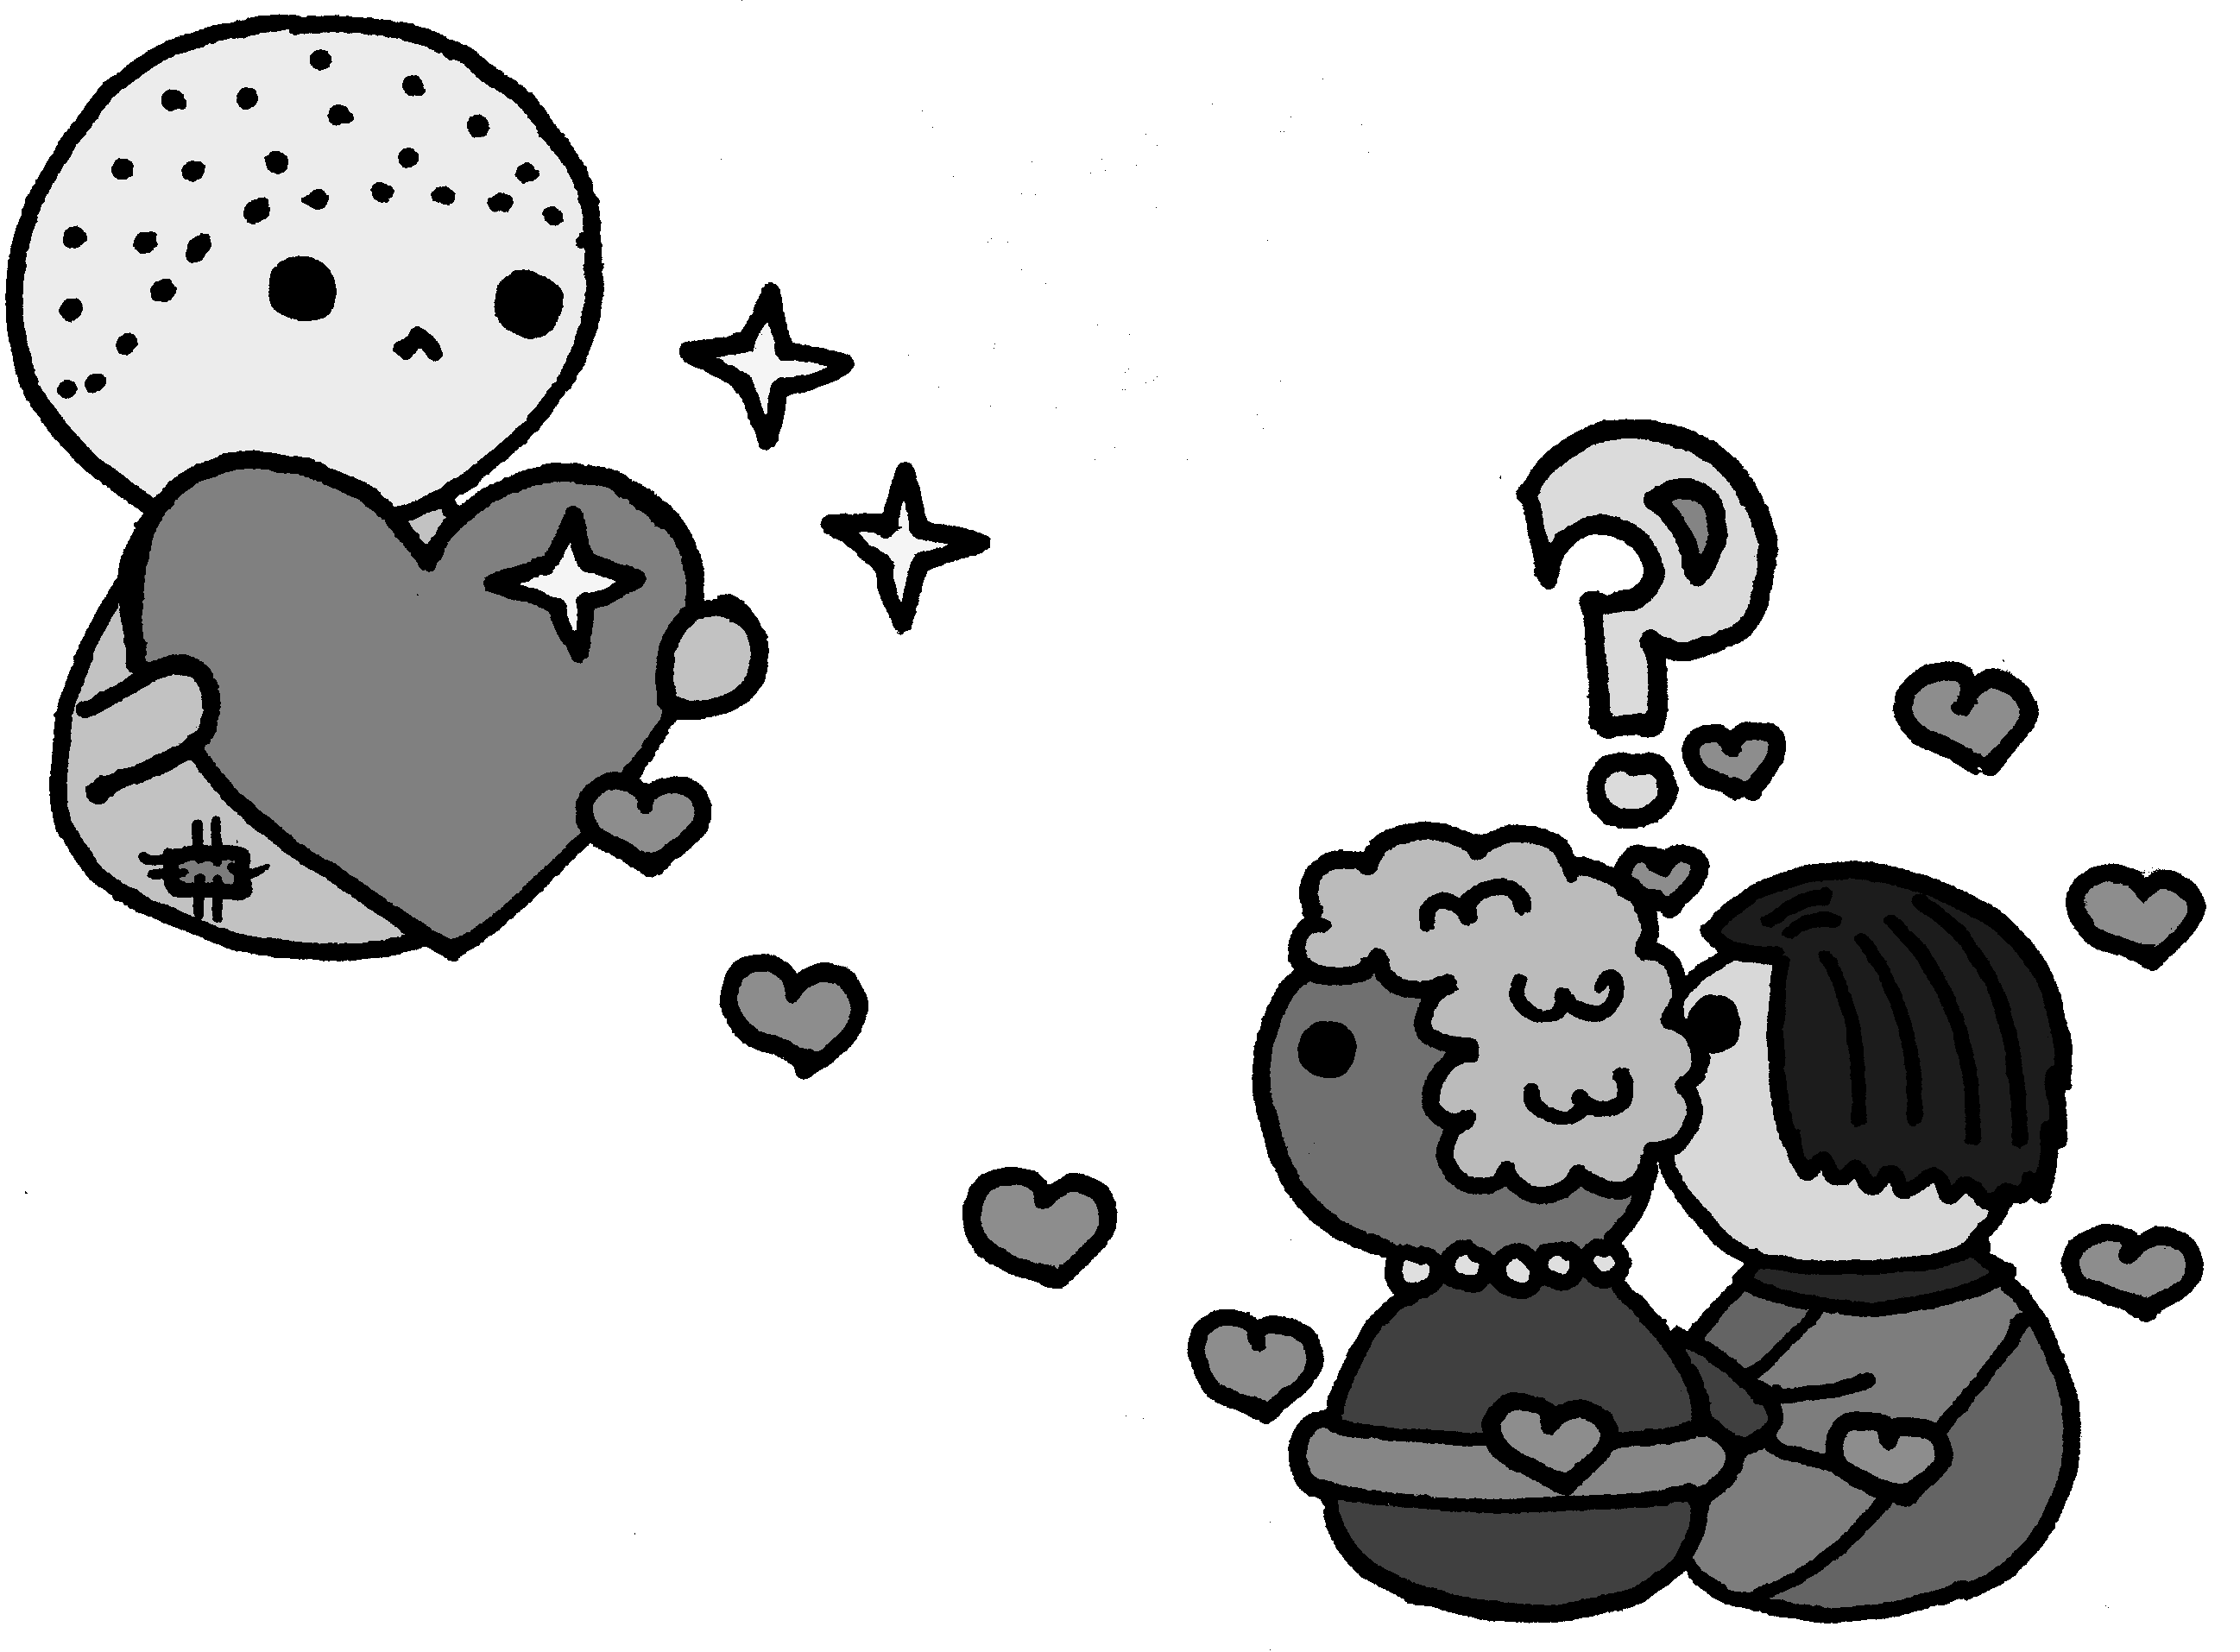
\includegraphics[width=0.6\paperwidth]{10bw.png}}
\end{figure}

\newpage
\thispagestyle{empty}
\begin{figure}[h]
    \centering
    \makebox[0pt]{%
    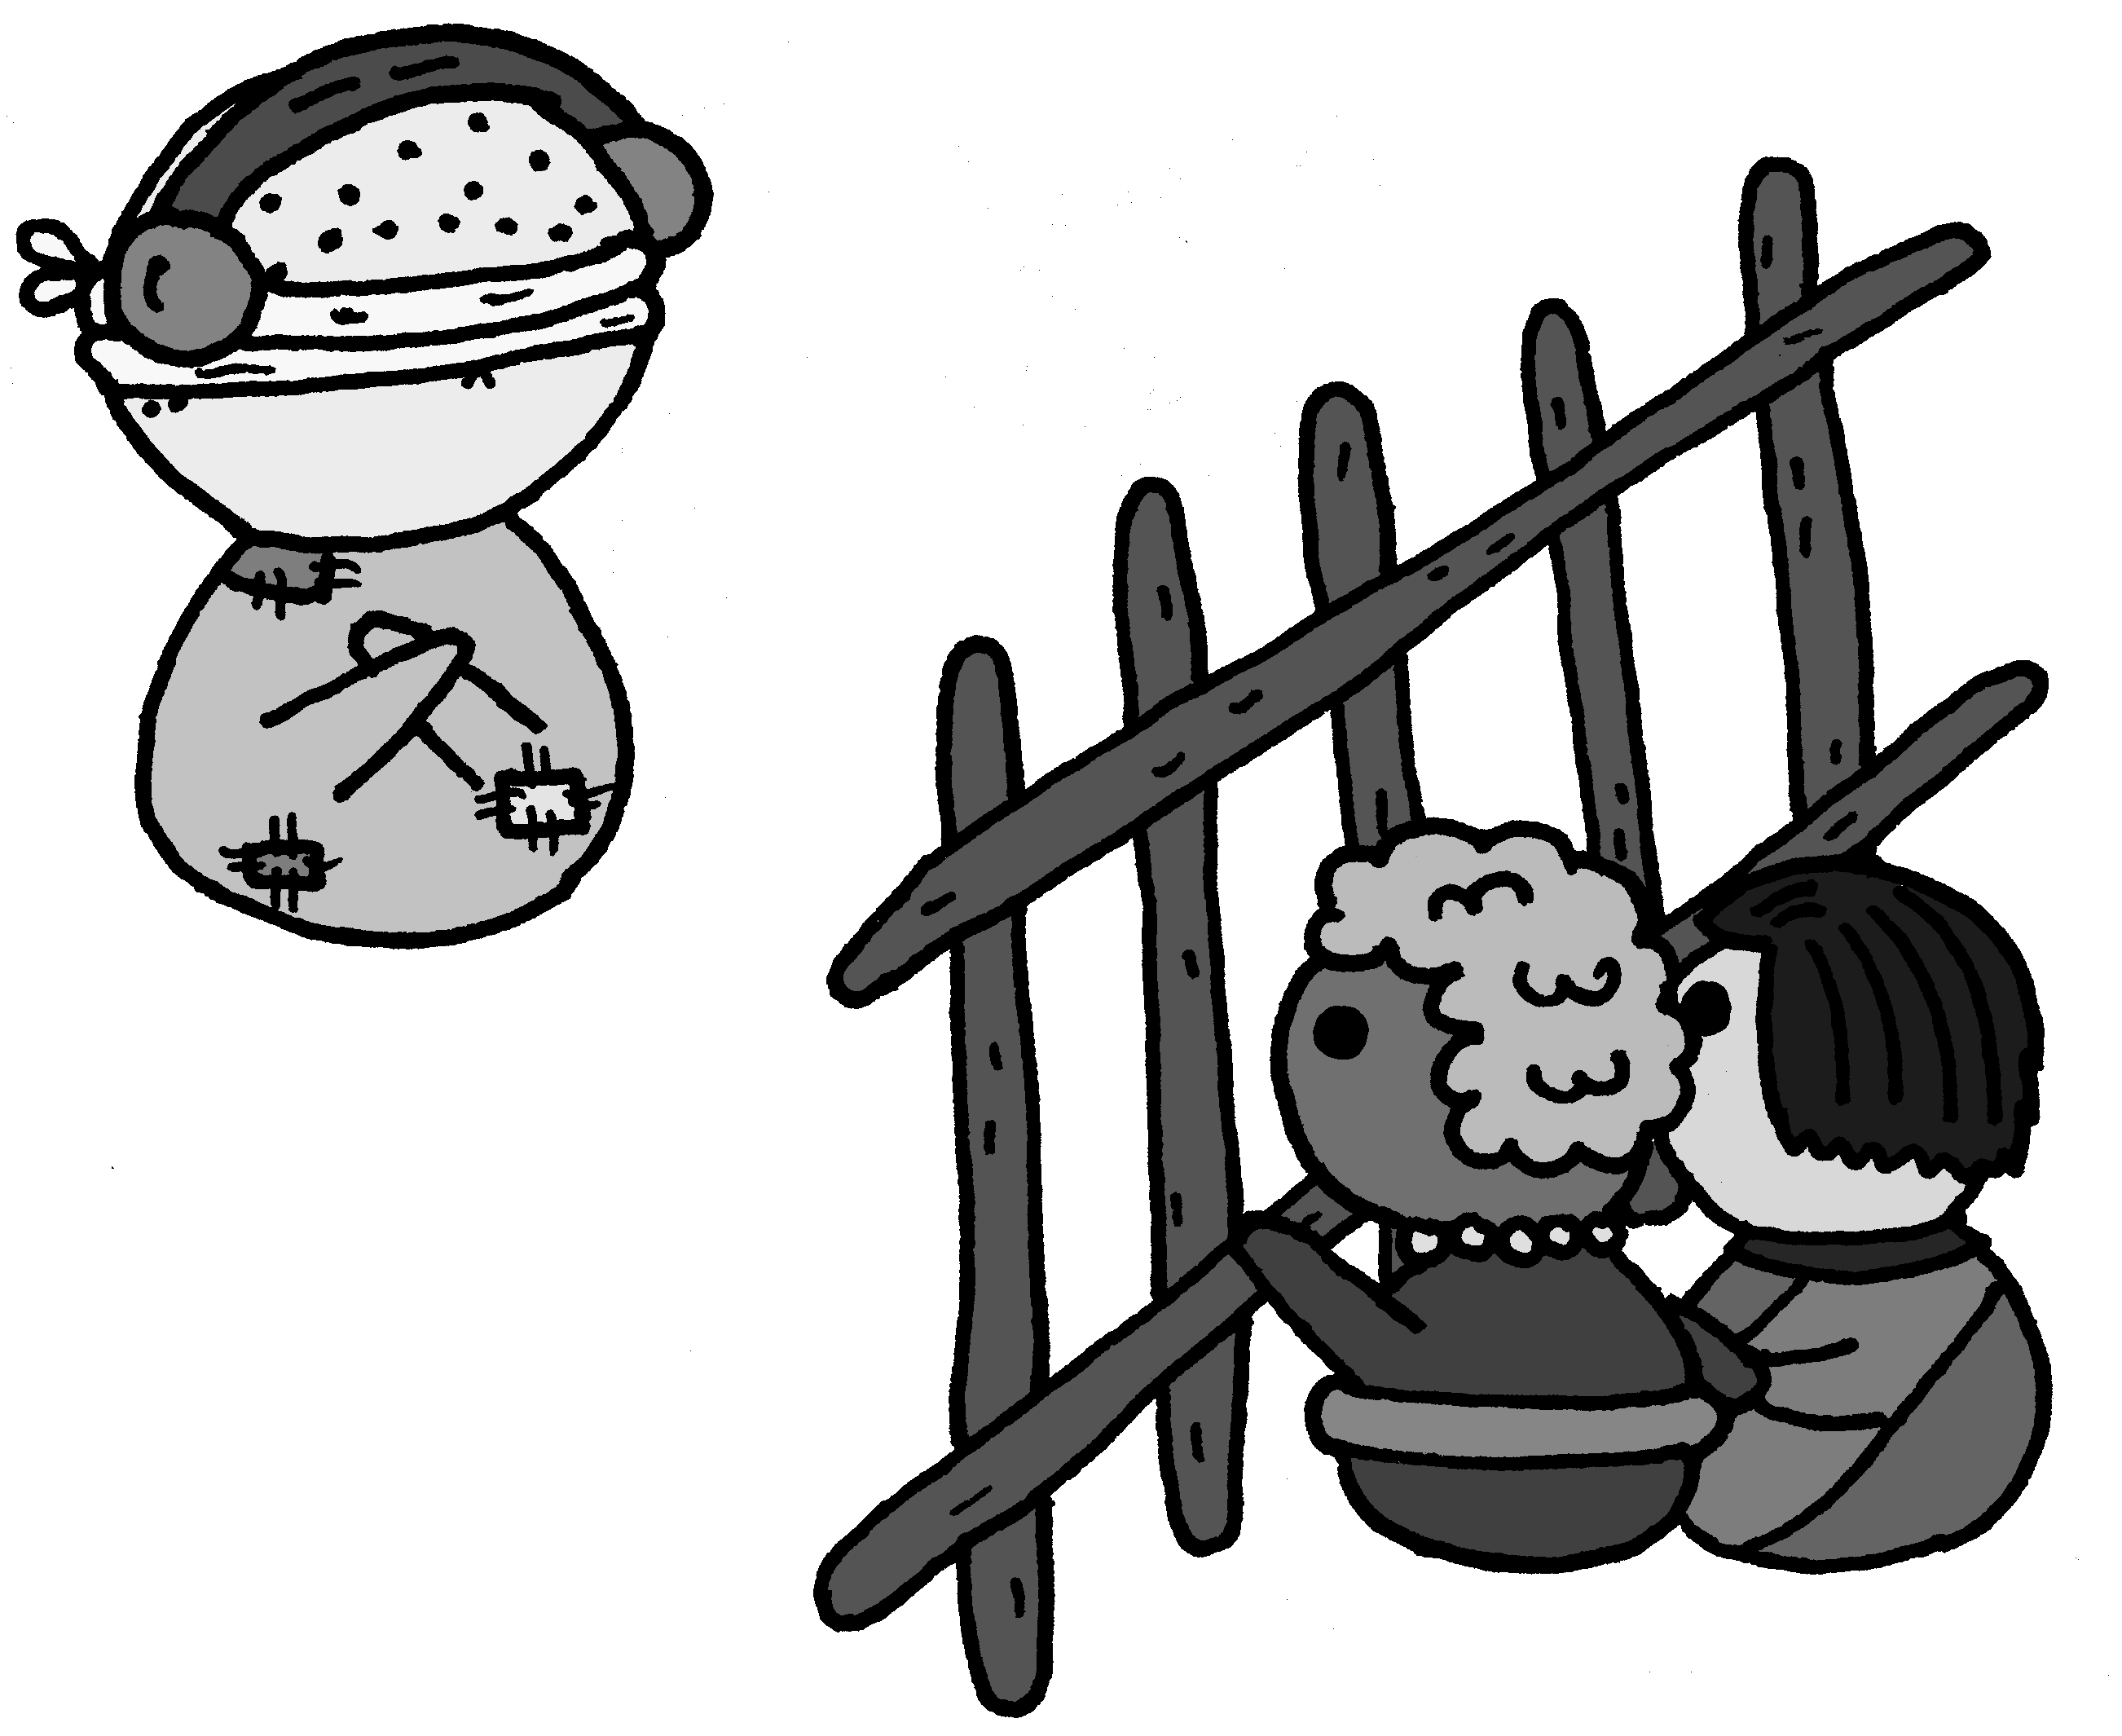
\includegraphics[width=0.8\paperwidth]{14bw.png}}
\end{figure}

\begin{quote}
\centering
\doublespacing
\textit{\Large \textbf{\textcolor{darkgray}{Si les bouddhistes et leurs organisations n’oeuvrent pas activement à l’inclusion, les personnes \mbox{LGBTQIA+} resteront toujours sur la touche.}}}
\end{quote}

\chapter*{Les obstacles à l’inclusion des personnes \mbox{LGBTQIA+}}
\addcontentsline{toc}{chapter}{Les obstacles à l’inclusion des personnes \mbox{LGBTQIA+}}
\markboth{Accueillir l’Arc-en-Ciel}{Les obstacles à l’inclusion des personnes \mbox{LGBTQIA+}}

\begin{wrapfigure}{r}{0.2\textwidth}
    \centering
    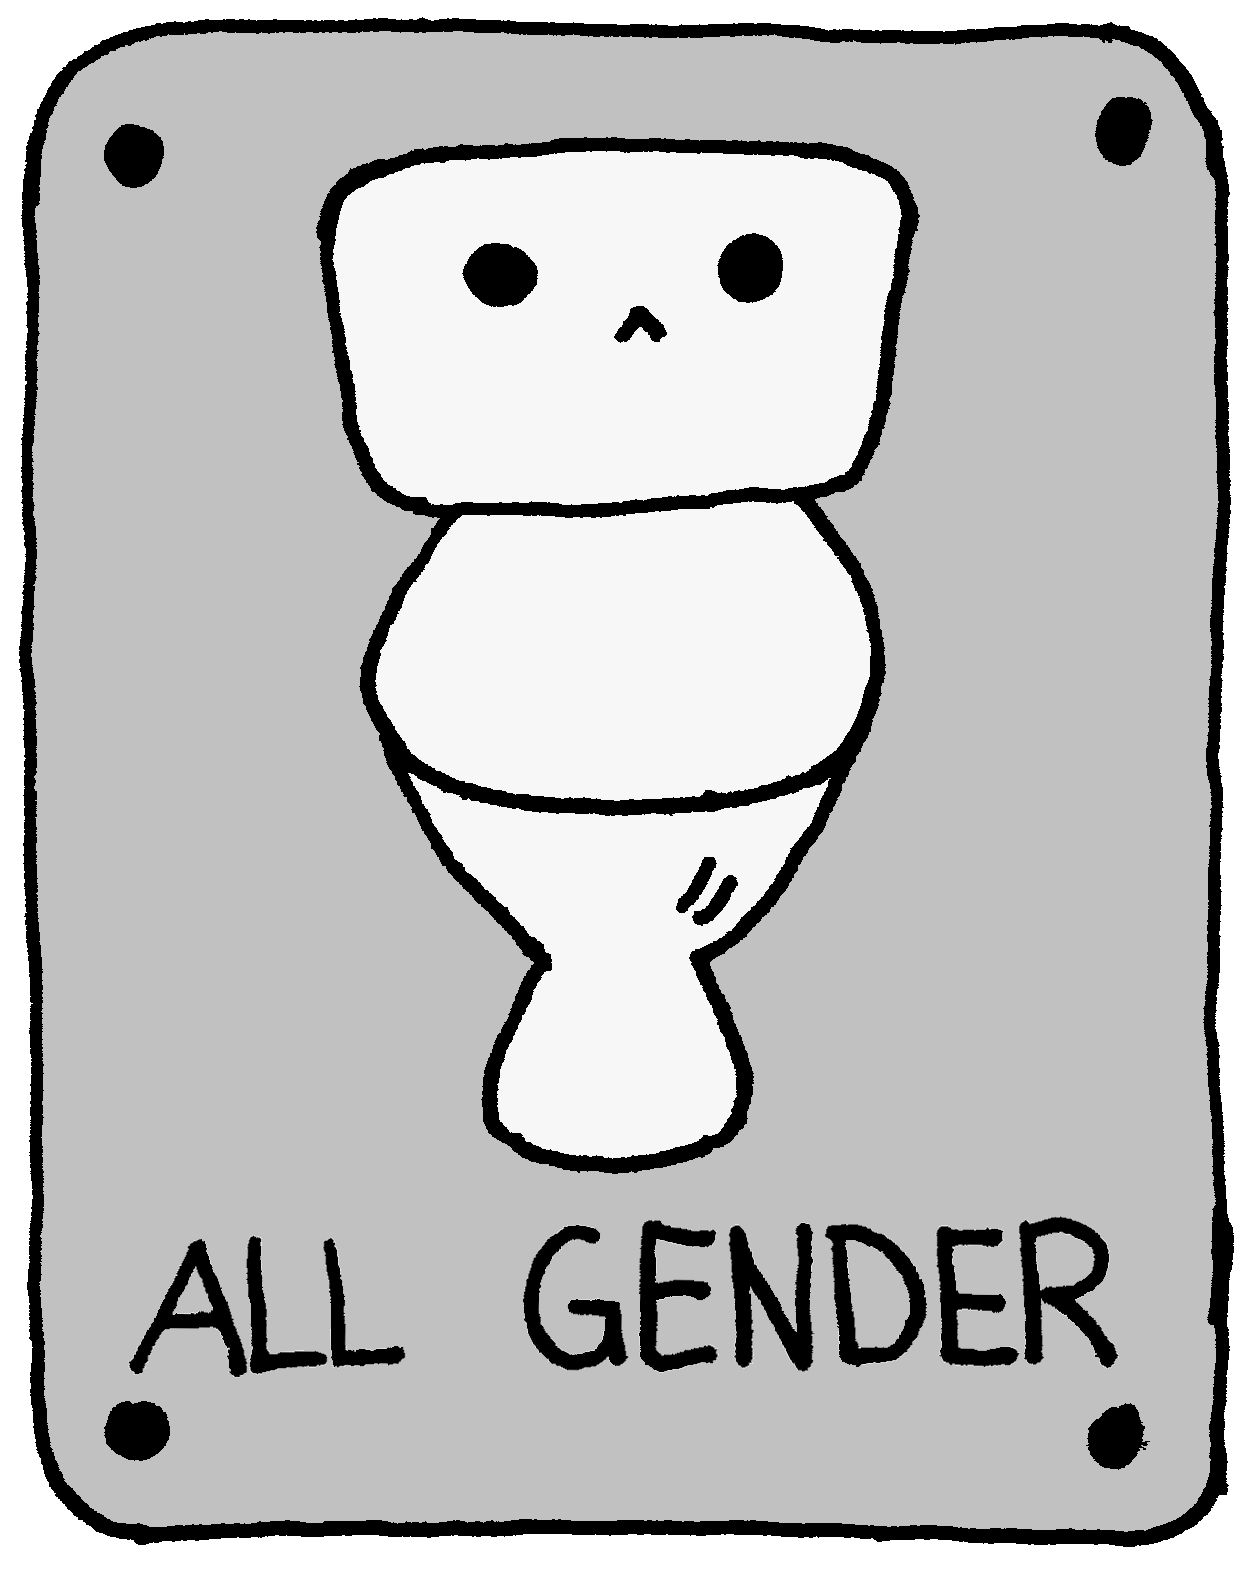
\includegraphics[width=0.2\textwidth]{16bw.png}
\end{wrapfigure}
La structuration et la gestion des organisations bouddhistes peuvent faire que des personnes se trouvent empêchées d’y participer. Pour prendre une analogie : les obstacles physiques, tels que les marches, peuvent exclure les personnes en fauteuil roulant, de sorte que l’on équipe les bâtiments de rampes et d’ascenseurs pour veiller à leur inclusion. De même, il existe des obstacles administratifs, physiques et conceptuels qui excluent les personnes \mbox{LGBTQIA+}. Il se peut que nous n’ayons pas conscience de ces obstacles, mais ils existent et ont des conséquences concrètes.

\begingroup
\begin{quote}
\doublespacing
\centering
\textit{\Large \textbf{\textcolor{darkgray}{Nous pouvons contribuer à éliminer les obstacles qui excluent les personnes \mbox{LGBTQIA+} et à créer des communautés bouddhistes plus sûres et plus inclusives.}}}
\end{quote}
\endgroup

\phantomsection
\section*{Les obstacles administratifs qui excluent}
\addcontentsline{toc}{section}{Les obstacles administratifs qui excluent}

\noindent Les formulaires d’inscription, les formulaires d’adhésion et les bases de données en ligne ne proposent souvent que les options \mbox{« homme »} ou \mbox{« femme »}. Cela exclut de nombreuses personnes transgenres, les personnes non binaires ainsi que certaines personnes intersexes qui préfèrent ne s’identifier ni comme homme ni comme femme. Le fait de ne prévoir que des options binaires indique à ces personnes qu’elles ne seront pas comprises ou bien accueillies avant même qu’elles ne se soient inscrites à une retraite ou abonnées à votre infolettre.

Pour faire preuve de plus d’inclusivité, ajoutez une option \mbox{« Autre »} aux formulaires qui posent la question du sexe et une case \mbox{« Mx »} ou \mbox{« Sans titre »} en plus de Mlle, Mme ou M. Le nom et le genre que certaines personnes utilisent au quotidien peuvent être différents de ce qui apparaît sur leurs documents d’identité officiels. Prévoyez donc la possibilité, pour les personnes, de préciser leur nom d’usage et demandez-leur quels pronoms elles souhaitent voir utilisés. Vérifiez aussi si le genre et les titres doivent absolument figurer sur certains formulaires ou si ces informations n’ont en fait aucune utilité.

\begin{figure}[h]
    \centering
    \makebox[0pt]{%
    
\includegraphics[width=0.25\paperwidth]{15bw.png}}
\end{figure}

\phantomsection
\section*{Les obstacles physiques qui excluent}
\addcontentsline{toc}{section}{Les obstacles physiques qui excluent}

\subsubsection*{Les espaces genrés}

\noindent Certains centres bouddhistes compartimentent leurs salles de méditation, salles à manger et autres espaces en zones genrées. Cette disposition peut même revêtir un caractère \mbox{« hiérarchique »}, les femmes étant assises derrière les hommes. Les espaces publics genrés ne sont pas adaptés à tous les membres de nos communautés et peuvent mettre certaines personnes mal à l’aise ou leur donner le sentiment d’être exclues.

Les espaces genrés attirent en outre une attention non désirée sur certaines personnes trans et font naître chez elles la peur d’être rejetées. Les personnes non binaires peuvent être angoissées à l’idée d’être obligées de décider où s’asseoir lorsque leur genre n’est pas reconnu. D’autres personnes n’apprécient pas ce type de ségrégation basée sur le genre parce qu’elle leur semble démodée et inutile.

\subsubsection*{Les toilettes}

\noindent Les personnes doivent se sentir suffisamment à l’aise pour utiliser les toilettes qui correspondent à leur identité de genre. Certaines personnes transgenres et non binaires préfèrent utiliser des toilettes non genrées plutôt que d’avoir à choisir entre des toilettes pour hommes et pour dames. Veiller à ce qu’il y ait des toilettes mixtes dans votre centre et lors des retraites aide les personnes d’identités de genre diverses à se sentir en sécurité et incluses.

\subsubsection*{L’hébergement en retraite}

\noindent Toute personne devrait se sentir à l’aise et avoir le sentiment d’être la bienvenue lors d’une retraite. Toutefois, pour de nombreuses personnes \mbox{LGBTQIA+}, les questions d’hébergement peuvent être une source d’angoisse. Elles peuvent en effet craindre d’être rejetées en raison de leur sexualité ou de se voir exclues en raison de leur genre, ou encore avoir le sentiment que leurs besoins ne sont tout simplement pas pris en compte.

Toutes les personnes, qu’elles soient cisgenres, transgenres ou non binaires, devraient pouvoir choisir le type d’hébergement qui correspond le mieux à leur identité de genre.
Étant donné que de nombreux centres de retraite scindent les structures d’hébergement en logements pour hommes et pour femmes, il est important que les organisations soient conscientes de leurs obligations légales en matière de non-discrimination à l’encontre des personnes trans qui utilisent ces espaces.

Des hébergements non mixtes seront toujours nécessaires. Toutefois, pour certaines personnes trans et non binaires, ces formules d’hébergement sont inadéquates, car elles ne tiennent pas compte du fait qu’il existe d’autres identités de genre ou que certaines personnes ne s’identifient pas au fait d’être un homme ou une femme. Pour faire preuve de davantage d’inclusivité et offrir des solutions plus sécurisantes, les organisateurs de retraites peuvent proposer un choix de dortoirs plus large : femmes, hommes et mixtes. Des formulaires d’inscription répertoriant ces options permettent aux personnes participantes de sélectionner celle qui leur convient le mieux.

Certaines personnes attirées par le même sexe préféreront peut-être être hébergées en dortoir mixte, car loger dans un dortoir réservé à un seul sexe pourrait se révéler être une expérience difficile pour elles. Leurs voisin.es de chambre pourraient en effet les faire se sentir importunes en raison de leur orientation sexuelle, ou le désir pourrait devenir une source de distraction.

Autant de raisons pour lesquelles un dortoir mixte offre une solution supplémentaire permettant aux personnes trans, non binaires et attirées par le même sexe de faire un choix plus adéquat pour elles. Une autre possibilité consisterait à offrir aux personnes \mbox{LGBTQIA+} la possibilité d’opter pour une chambre individuelle, afin de rendre leur expérience de retraite aussi confortable que possible.

L’accueil des personnes \mbox{LGBTQIA+} dans une retraite commence bien avant leur arrivée. Voici quelques exemples de choses que vous pouvez faire :

\begin{itemize}[label=\textbullet]
  \setlength\itemsep{-0.3em}
  \item Assurez-vous que la publicité indique qu’il s’agit d’un espace sûr et inclusif pour les personnes \mbox{LGBTQIA+}.
  \item Créez des formulaires d’inscription proposant des différentes options de genres, pronoms et préférences d’hébergement.
  \item Assurez-vous que les gestionnaires de retraite et les bénévoles soient sensibilisés aux pratiques d’inclusion des personnes \mbox{LGBTQIA+}.
  \item Mettez en place une signalisation pour créer des toilettes et des options d’hébergement mixtes
  \item Lors de la séance d’introduction à la retraite, rappelez aux personnes que ce lieu est un espace inclusif et accueillant pour tou.tes, y compris les personnes \mbox{LGBTQIA+}.
\end{itemize}

\bigskip
\bigskip

\begin{figure}[h]
    \centering
    \makebox[0pt]{%
    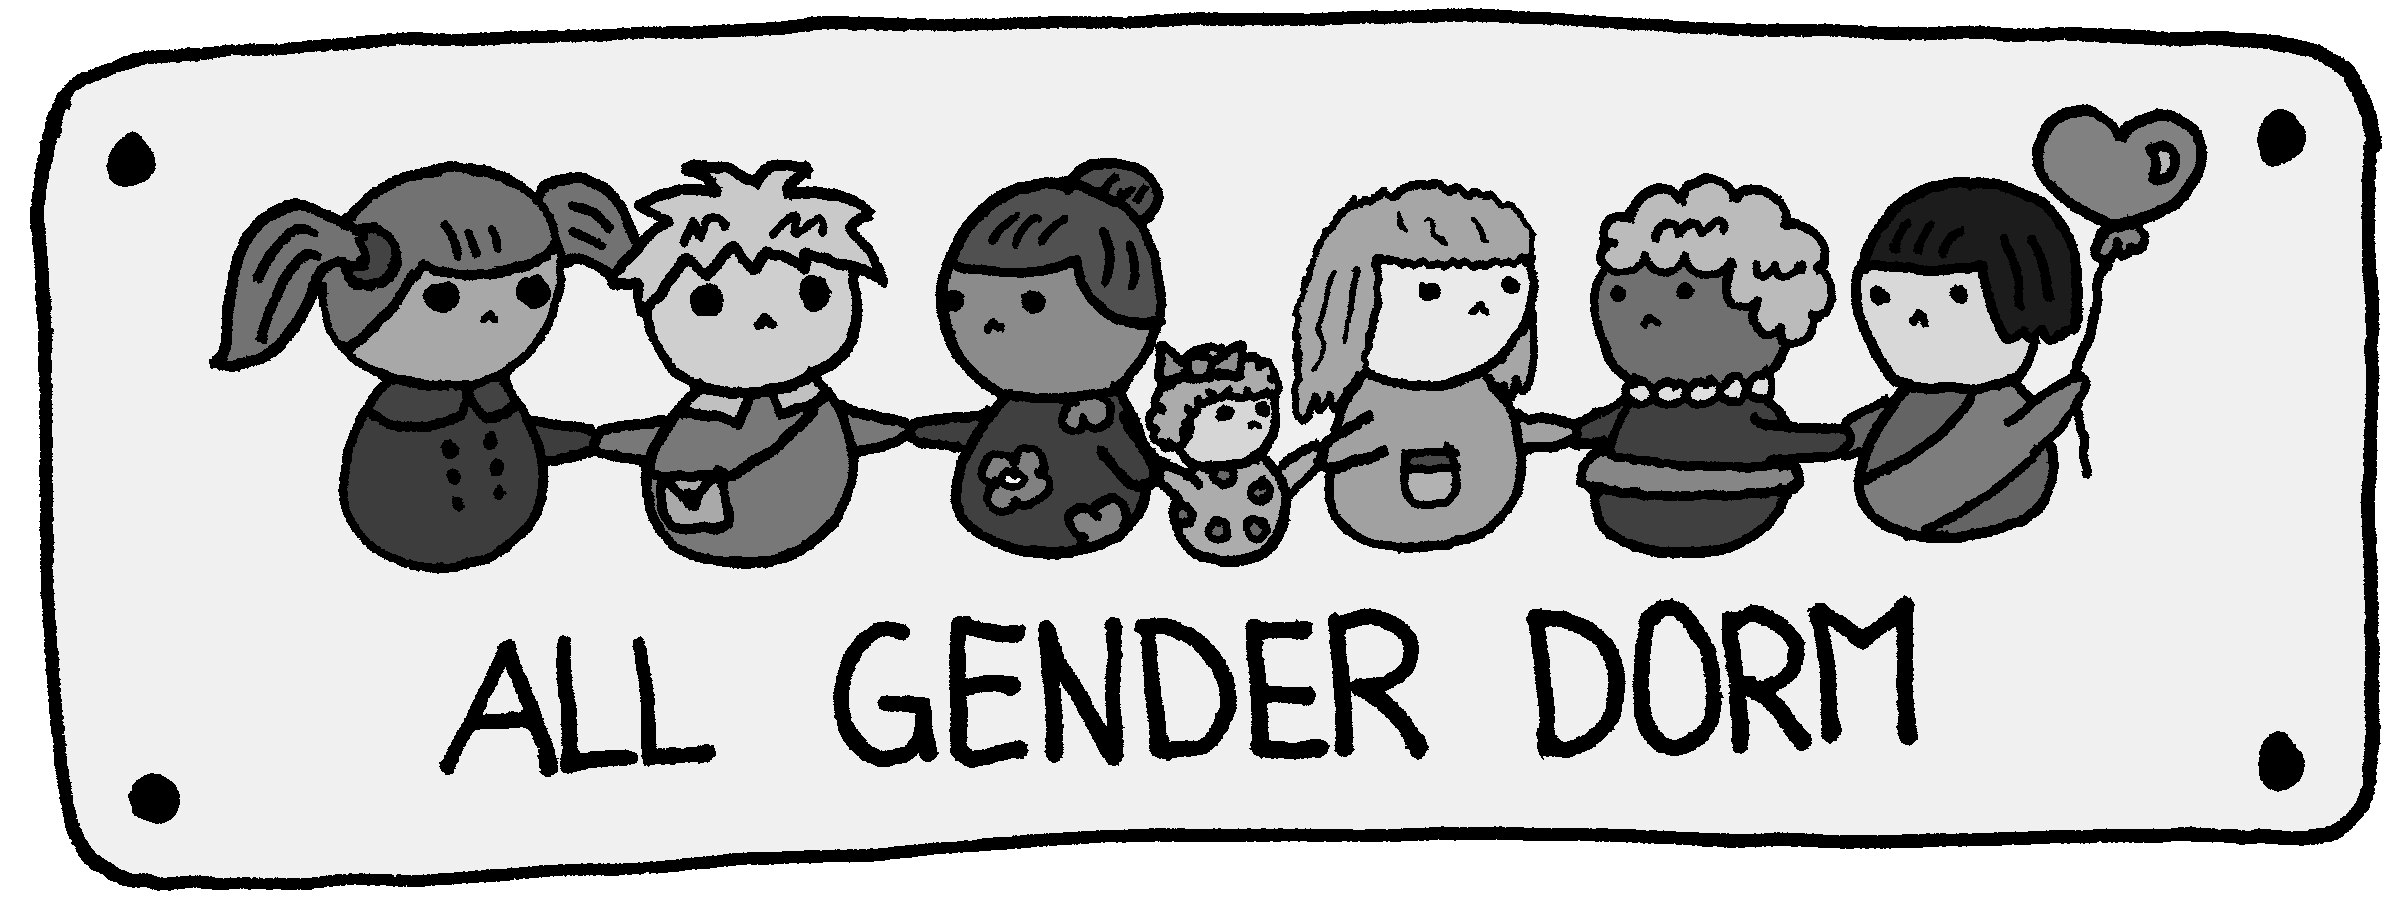
\includegraphics[width=0.8\paperwidth]{18-19bw.png}}
\end{figure}

\chapter*{Une parole qui fait du mal}
\addcontentsline{toc}{chapter}{Une parole qui fait du mal}
\markboth{Accueillir l’Arc-en-Ciel}{Une parole qui fait du mal}

\begin{figure}[h]
    \centering
    \makebox[0pt]{%
    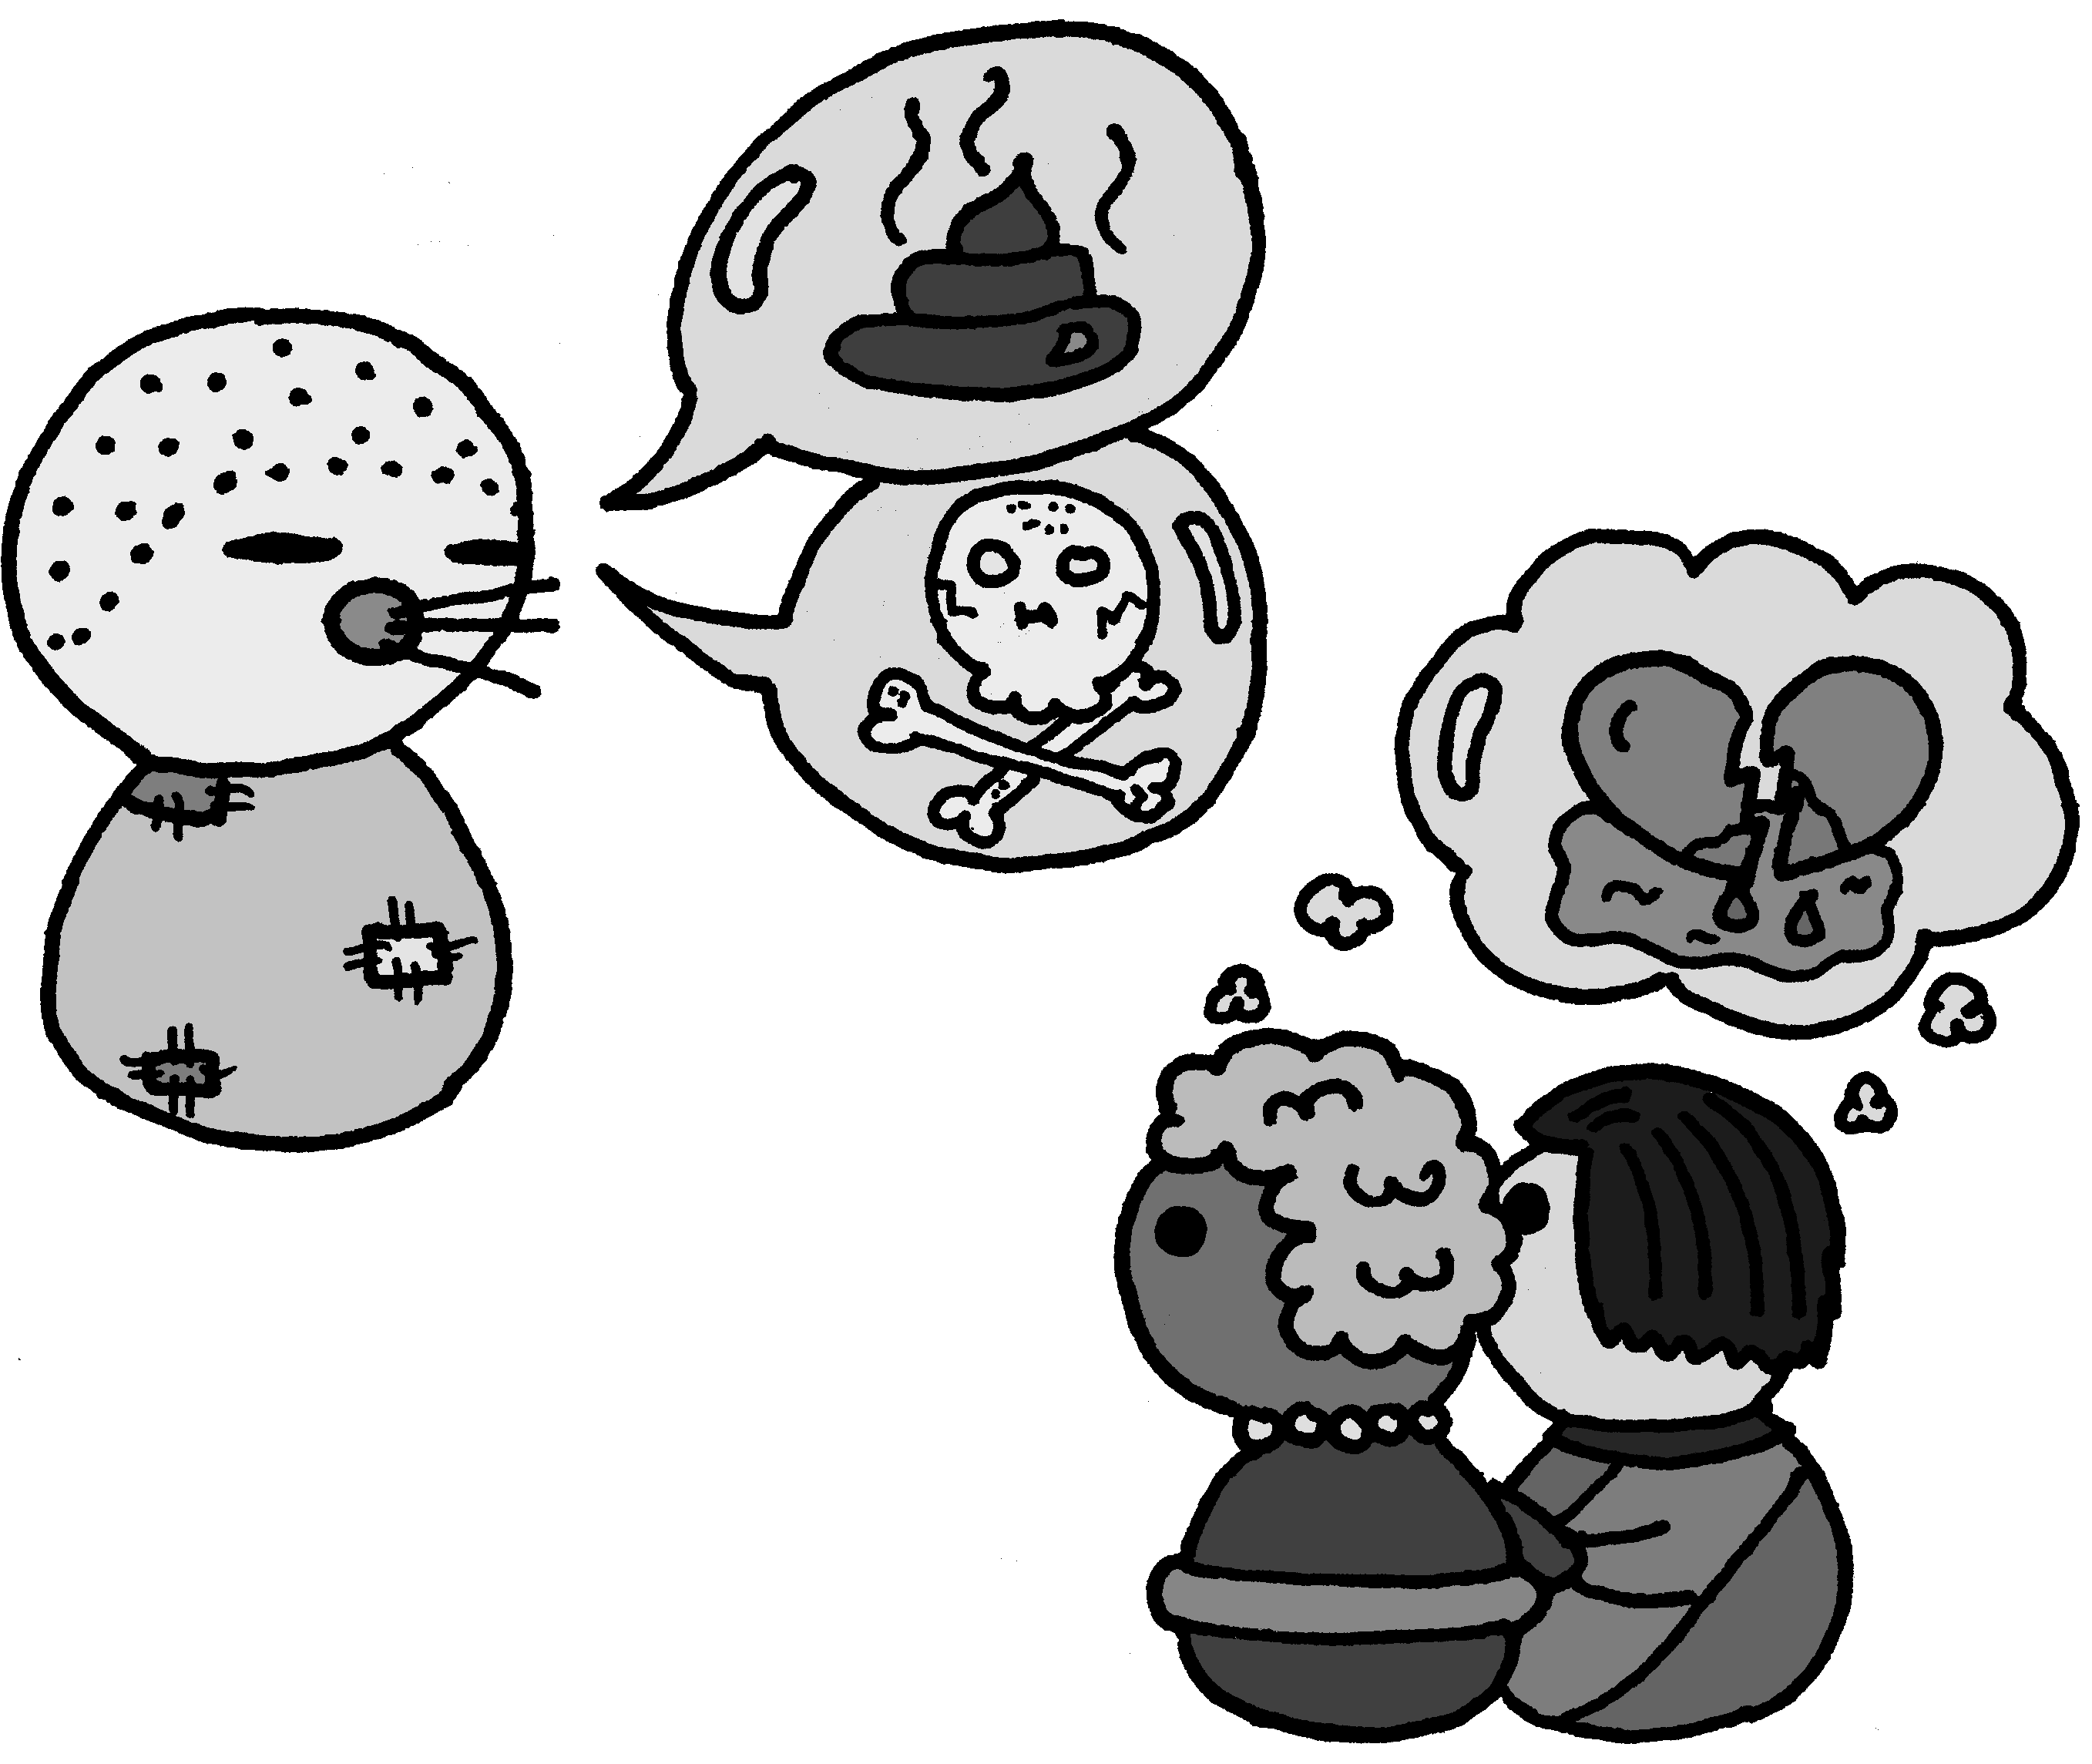
\includegraphics[width=0.3\paperwidth]{20bw.png}}
\end{figure}

\begingroup
\begin{quote}
\centering
\doublespacing
\textit{\Large \textbf{\textcolor{darkgray}{Nos paroles peuvent faire en sorte que chaque personne se sente en sécurité, respectée et incluse. Mais les paroles peuvent aussi contrarier, offenser et exclure.}}}
\end{quote}
\endgroup

\phantomsection
\section*{Des mots qui blessent}
\addcontentsline{toc}{section}{Des mots qui blessent}

\noindent La parole juste est un concept important dans le bouddhisme. Nos paroles ne sont pas sans conséquences. Des paroles bienveillantes ne causent aucun tort et témoignent du respect que nous portons aux personnes de notre communauté. Mais les paroles peuvent aussi blesser et faire en sorte que les personnes ne se sentent pas les bienvenues. Un langage irrespectueux, les blagues stupides et les questions indiscrètes ne relèvent pas de la parole juste et font la vie dure aux personnes \mbox{LGBTQIA+} désireuses de participer à nos communautés bouddhistes.

Voici quelques points importants à prendre en compte lorsque vous parlez avec des personnes \mbox{LGBTQIA+}.

\subsubsection*{Un langage irrespectueux}

\noindent Faites toujours preuve d’amabilité et prêtez attention aux mots susceptibles de blesser autrui. Un discours offensant peut également avoir des conséquences juridiques graves.

\begin{itemize}[label=\textbullet]
  \setlength\itemsep{-0.3em}
  \item Évitez d’utiliser des termes dépassés tels que \mbox{« transsexuel »}, \mbox{« travesti »} ou encore \mbox{« hermaphrodite »}. Ceux-ci ont des connotations médicales qui stigmatisent les personnes \mbox{LGBTQIA+}.
  \item N’utilisez pas de mots insultants tels que \mbox{« pédé »}, \mbox{« tapette »}, \mbox{« gouine »}, \mbox{« ladyboy »}, \mbox{« tante »}, \mbox{« travelo »} ou \mbox{« ça »}.
  \item Évitez les phrases qui dénigrent les personnes \mbox{LGBTQIA+}, telles que \mbox{« c}’est tellement ga\mbox{y »} ou \mbox{« o}n n’est pas des tapette\mbox{s »}.
\end{itemize}

\subsubsection*{Un langage qui exclut}

\noindent Prendre conscience de notre façon de nous exprimer est un bon moyen de faire de nos communautés bouddhistes des lieux où chaque personne se sent à sa place. Voici quelques conseils à cet égard :

\begin{itemize}[label=\textbullet, leftmargin=*]
\setlength\itemsep{-0.3em}
\item À un langage binaire de nature à exclure les personnes trans et non binaires, comme \mbox{« M}esdames et messieur\mbox{s »} ou \mbox{« C}hers frères et soeur\mbox{s »}, préférez des formules comme \mbox{« B}onjour à tout le mond\mbox{e »}.
\item Évitez d’employer un langage sexospécifique. Au lieu de \mbox{« l}’homme de la ru\mbox{e »}, essayez \mbox{« u}ne personne lambd\mbox{a »}. Au lieu de \mbox{« les gars »}, dites \mbox{« t}out le mond\mbox{e »}.
\item Veillez à ne pas exclure les personnes attirées par le même sexe. Au lieu de \mbox{« m}aris et femme\mbox{s »}, parlez de \mbox{« partenaires »}. Plutôt que de parler d’\mbox{« a}ttirance pour le sexe oppos\mbox{é »}, contentez-vous de parler d’\mbox{« attirance »}.
\item Ne réduisez jamais une personne à des parties de son corps ou à son orientation sexuelle. Au lieu de cela, rappelez-vous que vous avez en face de vous une personne à part entière et qu’elle ne se limite pas à ces choses. Ne décrivez pas quelqu’un en fonction de sa sexualité (\mbox{« c}e mec gay là-ba\mbox{s »}) ou de ses antécédents médicaux (\mbox{« c}’est un homme qui est devenu une femm\mbox{e »} ou \mbox{« i}l attend son opératio\mbox{n »})
\end{itemize}

\medskip

\begingroup
\begin{quote}
\centering
\textit{\large \textbf{\textcolor{darkgray}{Un langage inclusif permet à chaque personne de se sentir la bienvenue. Les formules d’exclusion tiennent certaines personnes à l’écart.}}}
\end{quote}
\endgroup

\subsubsection*{Des questions inappropriées}

\noindent Les questions indiscrètes portant sur la vie privée des personnes sont toujours inappropriées dans un contexte communautaire. Interroger quelqu’un sur ses organes génitaux, les procédures chirurgicales qu’iel a subies, son orientation sexuelle ou sa vie sexuelle est malvenu, car il s’agit de choses relevant de l’intime – et ce, pour tout le monde.
Quelques exemples de questions inappropriées :

\begin{itemize}[label=\textbullet]
  \setlength\itemsep{-0.3em}
  \item Tu es un garçon ou une fille ?
  \item Avez-vous été opéré.e ?
  \item Quel était votre nom avant votre transition ?
  \item Qui est l’homme dans votre couple ?
  \item Quelle position aimez-vous ?
  \item Avez-vous déjà couché avec quelqu’un du sexe opposé ?
  \item Mais si vous êtes bisexuel.le, pourquoi êtes-vous marié.e ?
\end{itemize}

\subsubsection*{Les faux compliments}

\noindent Complimenter quelqu’un en lui disant qu’iel a l’air hétéro ou cisgenre est insultant, car cela donne l’impression que ce serait mieux, en quelque sorte, que d’appartenir à la communauté \mbox{LGBTQIA+}. Ces idées reposent en outre sur des stéréotypes plutôt que sur une reconnaissance véritable de la diversité de notre communauté.
\begin{wrapfigure}{r}{0.25\textwidth}
    \makebox[150pt]{%
    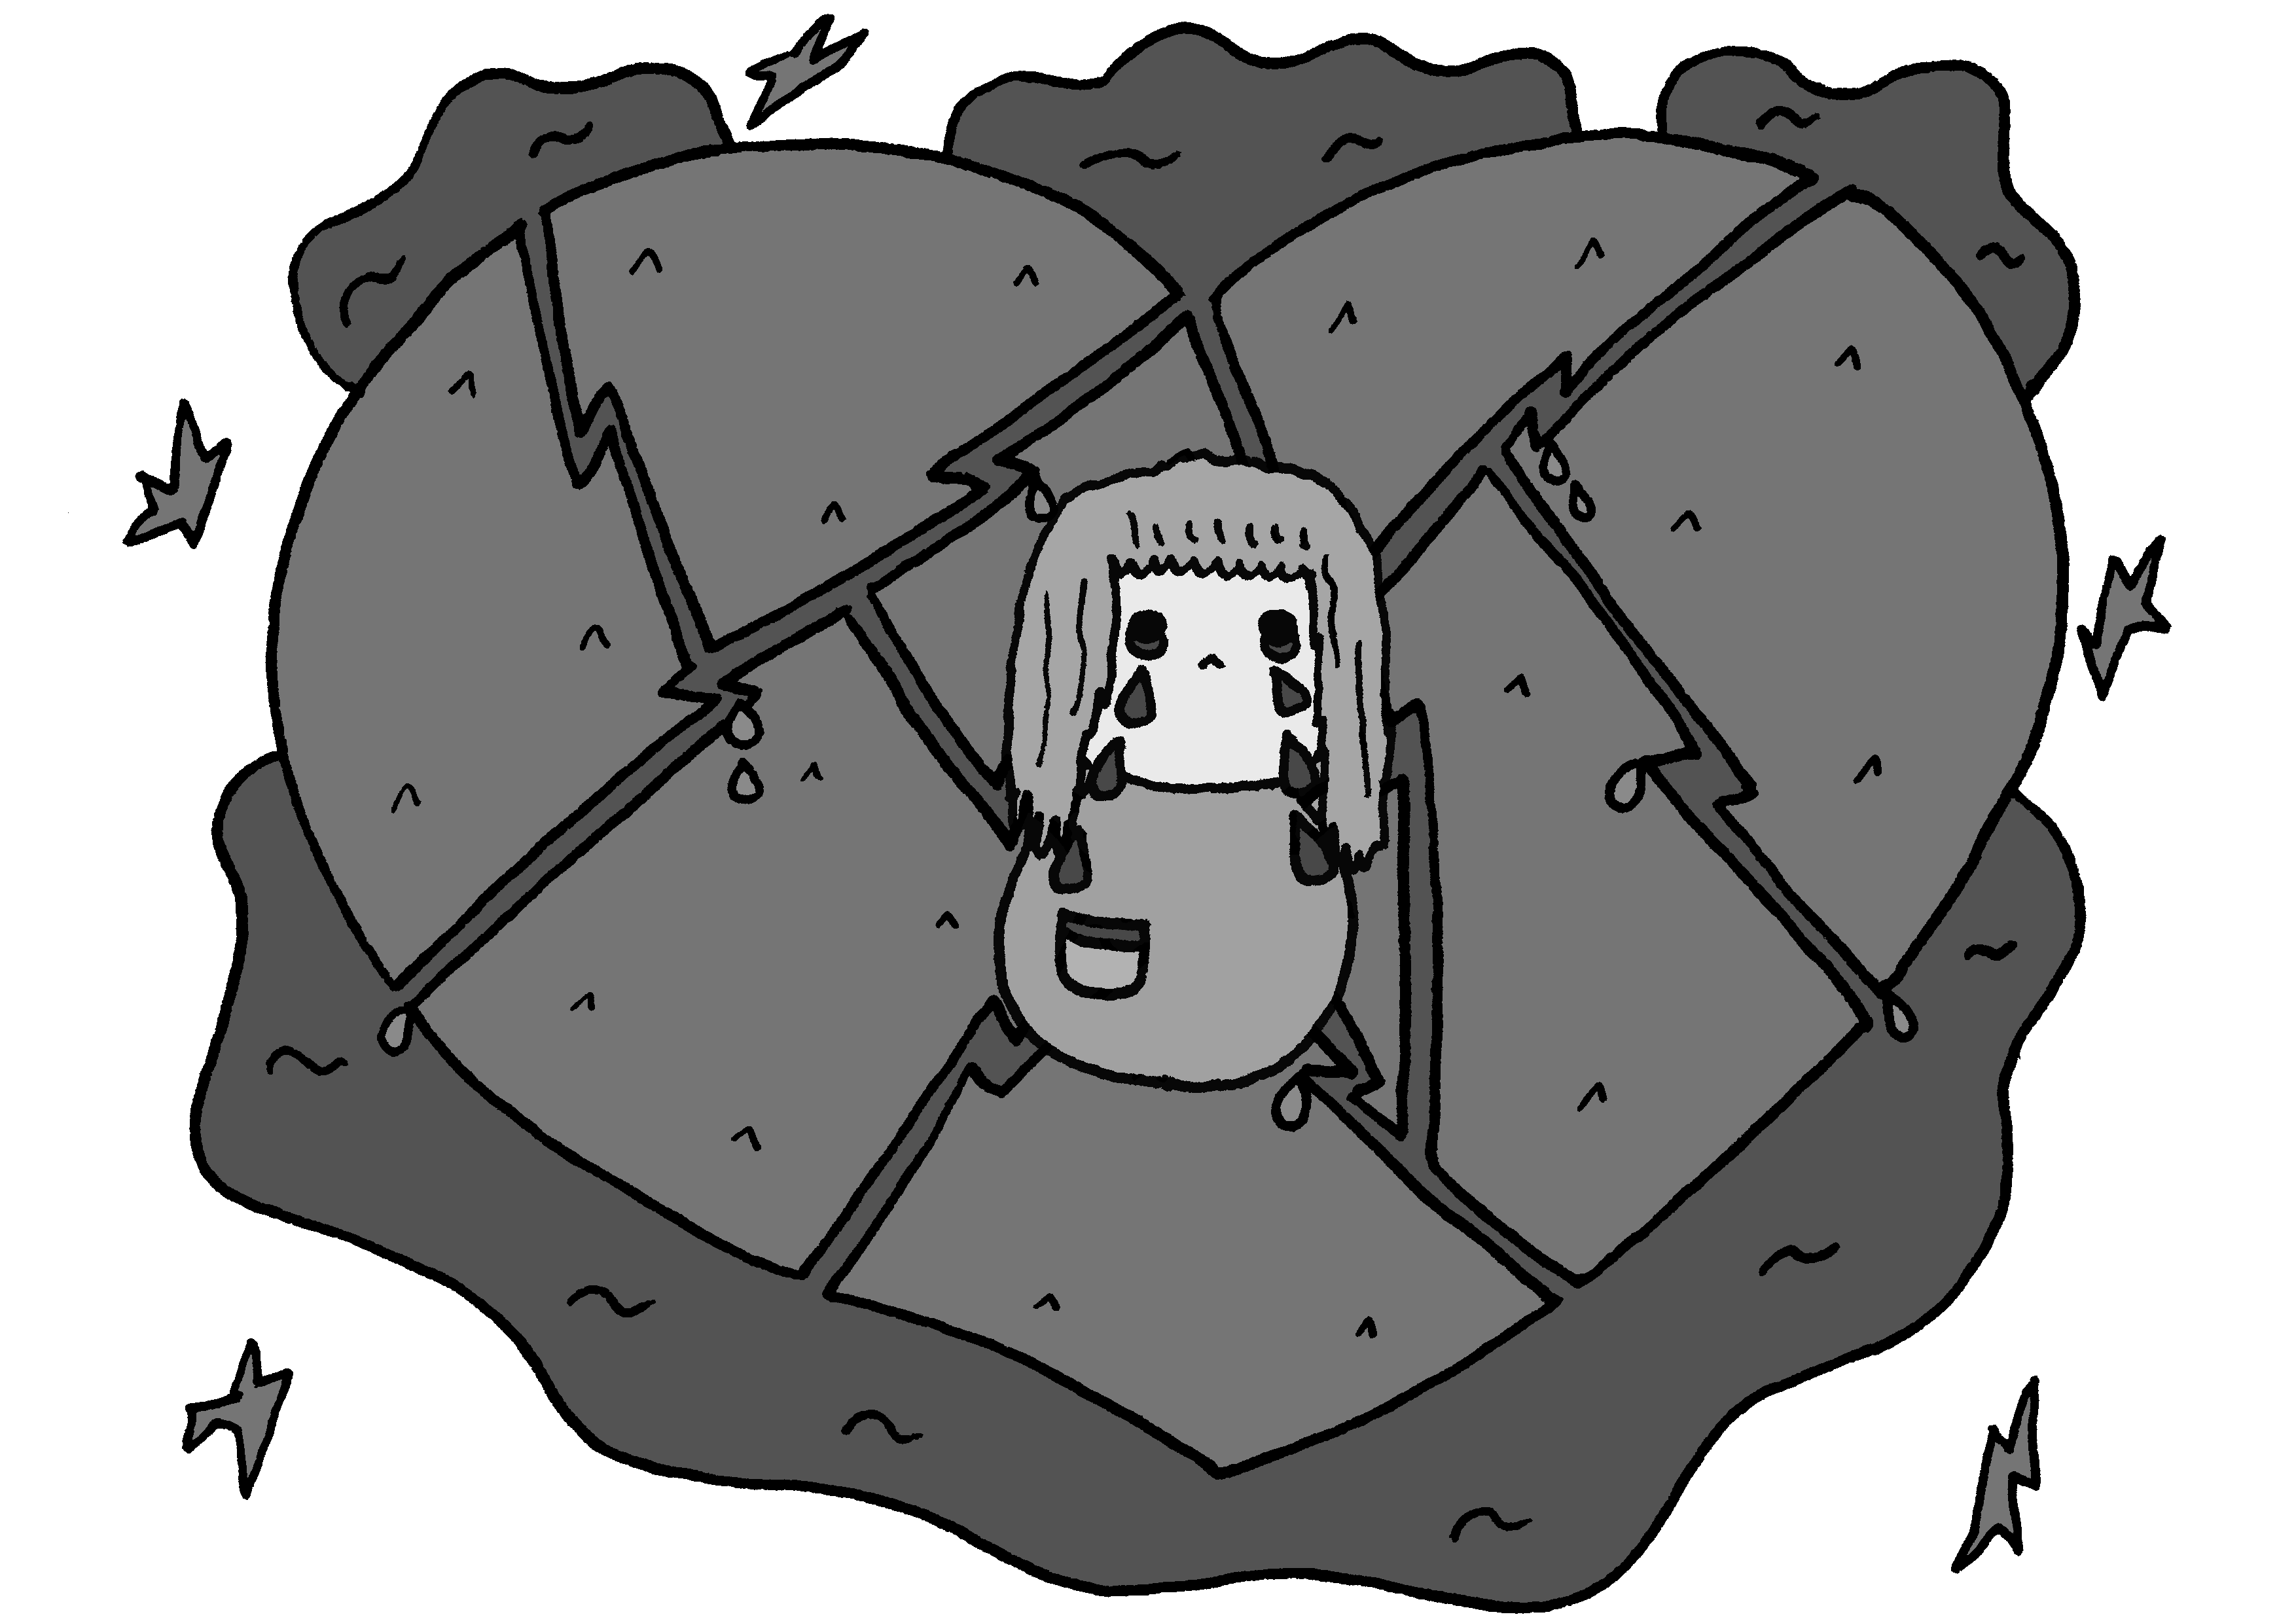
\includegraphics[width=0.25\textwidth]{29bw.png}}
\end{wrapfigure}
\begin{itemize}[label=\textbullet]
  \setlength\itemsep{-0.3em}
  \item Mais vous n’avez pas l’air gay !
  \item Je n’aurais jamais deviné que tu étais trans.
  \item Tu es plutôt viril pour un mec gay.
  \item Tu ne ressembles pas à une lesbienne.
\end{itemize}

\subsubsection*{Les blagues déplacées} 

\noindent Les choses drôles pour une personne peuvent être très blessantes pour une autre. Les blagues sur le genre, la sexualité ou le physique ne sont généralement pas drôles pour les personnes \mbox{LGBTQIA+}, parce qu’elles sont souvent utilisées pour les exclure, les intimider ou se moquer d’elles.

\subsubsection*{Les allusions grivoises}

\noindent Faire des gestes à caractère sexuel et des commentaires sur le genre, la sexualité ou le corps des personnes est toujours inapproprié dans les espaces communautaires.

\subsubsection*{Les stéréotypes}

\noindent Faire l’objet de clichés donne aux personnes l’impression de ne pas être considérées comme des individus à part entière. Rappelez-vous que les communautés \mbox{LGBTQIA+} sont des groupes très divers et que les personnes au sein de celles-ci ne sont pas toutes les mêmes ;
elles n’aiment pas toutes les mêmes choses et n’ont pas les mêmes centres d’intérêt.

\subsubsection*{Divulgation}

\noindent Ne divulguez pas l’orientation sexuelle ou l’histoire d’une personne sans sa permission (en clair, ne la \mbox{« s}ortez pas du placar\mbox{d »}). Les commérages de cet ordre sont susceptibles de blesser les personnes concernées et ne relèvent pas de la parole juste.

\phantomsection
\section*{L’importance des pronoms}
\addcontentsline{toc}{section}{L’importance des pronoms}

\noindent Nous apprécions tou.tes d’être reconnu.es et respecté.es pour ce que nous sommes.

Les pronoms sont des mots qui renvoient aux personnes, comme \mbox{« vous »}, \mbox{« nous »} ou \mbox{« ils »}. Certains pronoms contribuent également à décrire le genre d’une personne, comme \mbox{« il »}, \mbox{« lui »} ou \mbox{« elle »}. Bien utiliser les pronoms est toujours important et montre du respect pour la personne. Nous voulons tou.tes que les autres personnes utilisent les pronoms qui nous correspondent. C’est également vrai pour les personnes transgenres et de genre divers. Les pronoms font partie de l’identité d’une personne, au même titre qu’un nom.

Le pronom qu’une personne demande que l’on utilise pour la décrire reflète généralement son identité de genre. Le genre est un continuum. Certaines personnes peuvent avoir une apparence ou une voix qui ne correspondent pas à la façon dont elles s’identifient. Nous devrions donc ne pas préjuger des pronoms qu’utilise quelqu’un sur la seule base de son apparence ou de sa voix. Nous devrions plutôt demander discrètement à la personne ce qu’elle souhaite, puis utiliser ce pronom tant en sa présence qu’en son absence.

\subsubsection*{Types de pronoms}

\noindent Les pronoms conventionnels sont elle et il/lui. Certaines personnes ont une identité qui sort du cadre binaire masculin/féminin et utilisent des pronoms neutres, tels qu’iel/iels/cellui/celleux. D’autres personnes choisiront d’utiliser \mbox{« elle »} et \mbox{« il »} de manière interchangeable pour signaler que leur genre est fluide. D’autres encore préfèrent que l’on utilise uniquement leur prénom.

\subsubsection*{Utiliser les bons pronoms}

\noindent Nous pouvons faire un exemple du langage inclusif dans nos centres bouddhistes afin de montrer que nous comprenons l’importance d’utiliser les bons pronoms. Cela permettra aux personnes trans et de genre divers de se sentir mieux accueillies, comprises et incluses.
Rassurez-vous si vous ne maîtrisez pas ces nouveaux pronoms dans un premier temps. Il faut parfois un temps d’adaptation pour se les approprier, comme il nous en a fallu dans notre enfance pour nous approprier un langage nouveau.

\begin{itemize}[label=\textbullet]
\setlength\itemsep{-0.3em}
\item Présentez-vous en précisant les pronoms que vous utilisez pour vous-même.
\mbox{« Bonjour}, je m’appelle Bodhi. J’utilise le pronom \mbox{"elle". »}
\item Le cas échéant, demandez poliment et discrètement à la personne qui vous fait face quels pronoms elle s’applique. \mbox{« Bonjour}, mon nom est Lotus. J’utilise les pronoms iel/iels. Comment devrais-je vous appeler et vous \mbox{désigner ? »}
\item Utilisez toujours le nom et le pronom que la personne utilise actuellement, même si vous parlez d’elle dans le passé.
\item Informez les autres membres de votre communauté s’iels mégenrent une autre personne ou se trompent de prénom et aidez-les à mieux comprendre l’importance d’utiliser les bons noms et pronoms.
\item Ajoutez les pronoms que vous utilisez à votre signature électronique, à votre carte de visite, à votre profil d’enseignant.e ou à votre biographie : par exemple, Mitra Lovegood (elle), Comptabilité.
\end{itemize}

Ne perdez pas de vue que tout le monde ne voudra pas partager ses pronoms et que personne ne devrait être obligé de le faire.

\phantomsection
\section*{Mégenrage}
\addcontentsline{toc}{section}{Mégenrage}

\noindent Le mégenrage consiste à désigner une personne ou à s’adresser à elle en utilisant un genre qui ne correspond pas à celui auquel elle s’identifie ou identifie son corps. Parler d’une personne comme elle le souhaite est la moindre des politesses. Le mégenrage est blessant et donne aux personnes le sentiment de ne pas être respectées, reconnues ou acceptées. Il les fait se sentir rejetées.

Demander à une personne les pronoms qu’elle utilise et les employer correctement est un moyen simple de témoigner du respect pour son identité de genre. Dans le doute, utilisez les pronoms neutres iel/iels jusqu’à ce que vous connaissiez le genre de la personne, puis employez les pronoms ad hoc. Si quelqu’un s’identifie comme une femme ou un homme, n’utilisez pas de pronoms neutres – utilisez les pronoms correspondant à son genre lorsque vous parlez de la personne.

Si vous vous trompez, ce n’est pas grave ! Cela peut arriver ! Si vous vous trompez de pronom, excusez-vous tout de suite, utilisez le bon pronom et passez à autre chose sans en faire tout un plat. Si vous vous rendez compte de votre erreur plus tard, excusez-vous en privé et passez à autre chose.

\subsubsection*{Ménommage}

\noindent Les prénoms sont importants pour nous tou.tes. Bien nommer quelqu’un est une question de courtoisie élémentaire. Ménommer quelqu’un consiste à appeler une personne trans par le prénom qu’elle utilisait avant sa transition. Ce peut être extrêmement blessant et contrariant pour les personnes trans. Ne demandez jamais à une personne de vous révéler son ancien prénom. Lorsqu’une personne décide d’affirmer son identité en utilisant un nouveau prénom, nous devrions utiliser celui-ci pour lui témoigner notre respect et notre soutien.

\phantomsection
\section*{Des instructions inconfortables}
\addcontentsline{toc}{section}{Des instructions inconfortables}

\noindent Les enseignant.es de méditation doivent être conscient.es que certaines personnes trans se sentent très mal à l’aise dans leur corps. On parle parfois à cet égard de \mbox{« d}ysphorie de genr\mbox{e »}. Il s’agit d’un sentiment de détresse associé à une incongruence entre l’identité de genre de la personne et le sexe qui lui a été attribué à la naissance. Si un.e méditant.e souffre d’une dysphorie de genre, utilisez des techniques de méditation qui ne se concentrent pas sur les zones problématique de son corps. Si quelqu’un est aux prises avec une dysphorie portant sur sa poitrine, suggérez une marche en méditation, ou la méditation de l’amour bienveillant, ou toute autre forme de méditation qui ne se focalisera à aucun moment sur sa poitrine.

Dans le cadre d’une séance de méditation collective, il peut être utile de proposer plusieurs techniques. C’est particulièrement important si les personnes débutent la méditation et sont pas rodées à gérer les sensations ou les émotions désagréables.

Les enseignant.es ne doivent pas non plus oublier d’utiliser un langage qui inclue des personnes présentant des identités de genre, des orientations sexuelles et des corps différents, et ne pas simplement partir du principe que toutes les personnes qui participent à la retraite sont hétérosexuelles ou cisgenres.

\bigskip

\begin{figure}[h]
    \centering
    \makebox[0pt]{%
    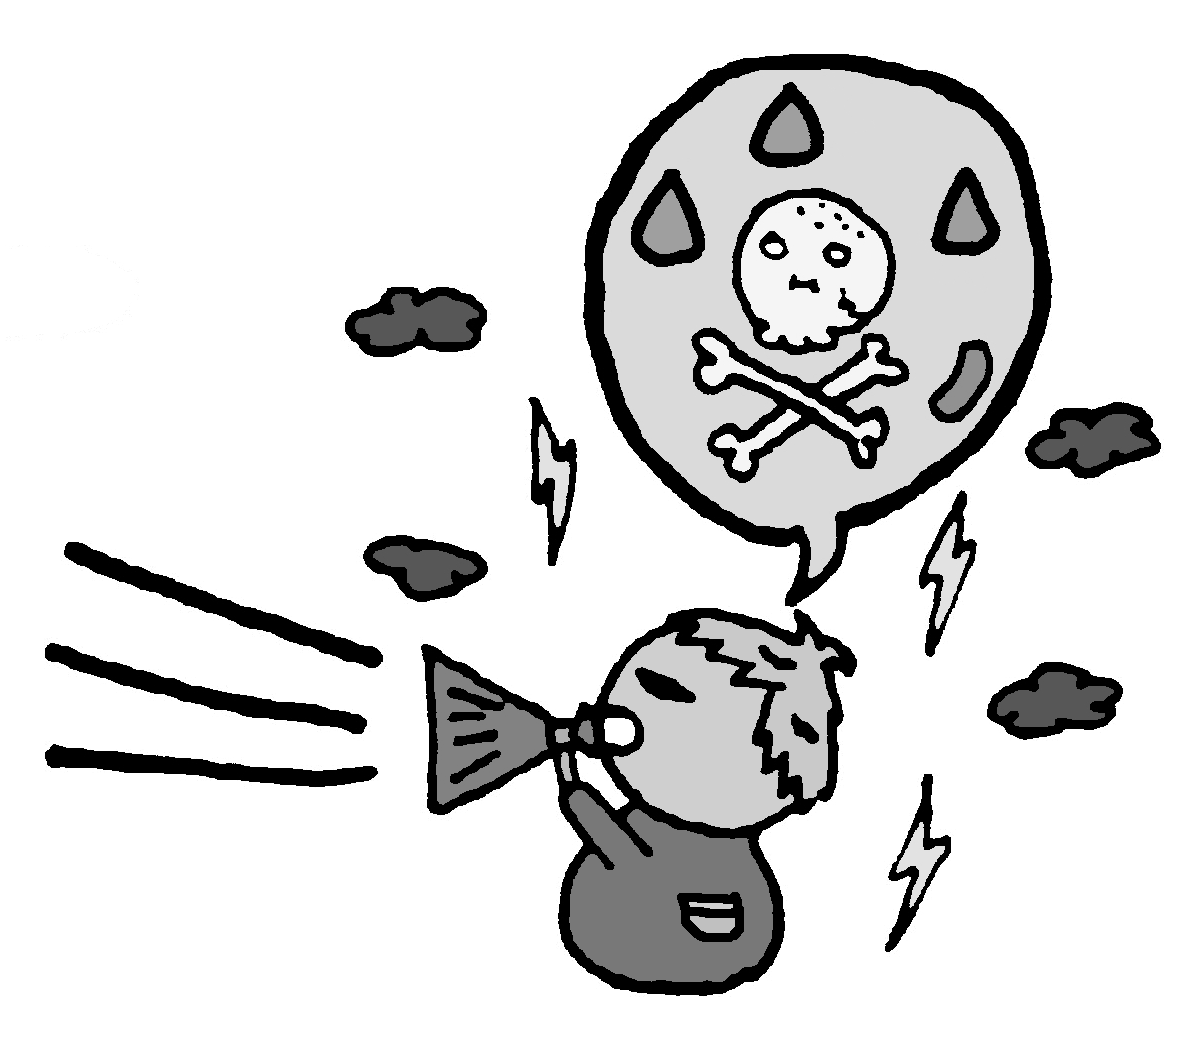
\includegraphics[width=0.4\paperwidth]{22bw2.png}}
\end{figure}

\begingroup
\begin{quote}
\centering
\doublespacing
\textit{\Large \textbf{\textcolor{darkgray}{Les opinions d’autrui peuvent être une source de préjugés et d’intolérance, de discrimination et d’oppression, ainsi que de haine et de violence à l’égard des communautés \mbox{LGBTQIA+}.}}}
\end{quote}
\endgroup

\chapter*{Les vues qui nuisent}
\addcontentsline{toc}{chapter}{Les vues qui nuisent}
\markboth{Accueillir l’Arc-en-Ciel}{Les vues qui nuisent}

\phantomsection
\section*{La pénible réalité de la discrimination}
\addcontentsline{toc}{section}{La pénible réalité de la discrimination}

\noindent Bien que la plupart des personnes \mbox{LGBTQIA+} aient une vie saine et heureuse, des études montrent qu’un nombre disproportionné d’entre elles affichent une moins bonne santé mentale et présentent un risque accru de comportements suicidaires. Ce phénomène est directement lié à la stigmatisation, aux préjugés, à la discrimination et à la maltraitance auxquels elles font face juste parce qu’elles sont LBGTQIA+.

Partout dans le monde, les personnes \mbox{LGBTQIA+} sont en outre confrontées à des actes d’intimidation, mais aussi à des violences verbales et physiques. Autant de raisons bien réelles et impérieuses pour lesquelles il nous faut continuer à parler des discriminations et des préjugés dont les personnes \mbox{LGBTQIA+} sont victimes et comprendre les défis auxquels elles font face, de manière à pouvoir créer des espaces qui soient sûrs et accueillants pour tout.es.

\noindent\fbox{%
   \parbox{\textwidth}{%
\textit{\textbf{\Large Discrimination à l’encontre des personnes \mbox{LGBTQIA+}}}

\begin{itemize}[label=\textbullet]
\item 72 pays considèrent les relations sexuelles librement consenties entre hommes comme une infraction pénale.
\item 44 pays pénalisent les relations sexuelles librement consenties entre femmes.
\item Les relations sexuelles consenties entre personnes de même sexe sont passibles de la peine de mort dans onze pays.
\item Quinze pays criminalisent l’identité de genre des personnes transgenres par le biais de lois sur le \mbox{« travestissement »}, l’\mbox{« u}surpation d’identit\mbox{é »} et la \mbox{« dissimulation »}.
\item Partout dans le monde, des personnes intersexes subissent des interventions médicales forcées qui violent leurs droits humains et leur intégrité physique.
\end{itemize}
   }
}

\phantomsection
\section*{Quelques mots sur le non-soi}
\addcontentsline{toc}{section}{Quelques mots sur le non-soi}

\noindent Certain.es bouddhistes accusent injustement les personnes \mbox{LGBTQIA+} d’être \mbox{« obsédées »} par leur identité ou de \mbox{« s’accrocher »} à une certaine idée d’elles-mêmes. Iels mettent en avant la doctrine bouddhiste de l’anatta (non-soi) et insistent sur le fait que ces identités sont illusoires et n’existent pas réellement. Ou iels prétendent que se concentrer sur une identité est contraire à l’enseignement bouddhiste et que c’est pour cela que les personnes \mbox{LGBTQIA+} souffrent.

Cependant, il est important de se rappeler qu’être homosexuel.le, trans ou intersexe constitue un élément fondamental de l’être humain. Suggérer que ces facettes d’une personne ne seraient en quelque sorte pas réelles, ou pas importantes, est une vue erronée et un détournement de la doctrine bouddhiste. C’est nier la réalité de l’expérience vécue par les personnes et gommer des parties importantes de leur vie, comme leurs relations, leur communauté ou leur travail. Une telle approche est également néfaste car elle tend à minimiser les discriminations, les préjugés et les violences très réels que les personnes \mbox{LGBTQIA+} subissent chaque jour.

Certain.es bouddhistes utilisent le concept de non-soi pour réduire au silence les personnes \mbox{LGBTQIA+} qui parlent de problèmes qui les affectent, ou de la souffrance bien réelle qu’elles vivent. Les personnes \mbox{LGBTQIA+} souffrent principalement à cause de l’attitude d’autrui envers leur identité, mais le fait d’être \mbox{LGBTQIA+} n’est en soi pas plus une cause de souffrance que d’être cisgenre ou hétérosexuel.le. Les personnes \mbox{LGBTQIA+} parlent d’identité parce qu’elles sont souvent socialement affectées par des attitudes discriminatoires et veulent voir changer ces aspects préjudiciables de la société. Le genre et la sexualité sont importants pour les personnes et pour la société. Nous devrions célébrer notre diversité, plutôt que d’ignorer ou de gommer ces aspects.

Il est donc essentiel que les bouddhistes réfléchissent soigneusement à la façon dont iels parlent du non-soi aux personnes victimes d’oppression en raison de leur identité. Faute de quoi, au lieu d’être un outil utile pour évoluer sur un plan personnel, le non-soi peut devenir une arme qui nuit à autrui. Cet \mbox{« a}natta instrumentalis\mbox{é »} peut se muer en une autre attaque injuste à l’encontre des personnes \mbox{LGBTQIA+}.

\subsubsection*{Qui êtes-vous ?}

\noindent On critique parfois les personnes \mbox{LGBTQIA+} parce qu’elles parlent des problèmes qui les affectent, et on leur dit qu’elles sont obsédées par leur identité. Lorsque l’on parle du non-soi, il est important de se rappeler que les personnes cisgenres et hétérosexuelles ont également une identité de genre et sexuelle. Peut-être est-il plus difficile de le voir parce que ces groupes se considèrent souvent comme \mbox{« normaux »}, et que la société tend à fortement renforcer leur identité d’une manière dont ils peuvent ne pas avoir conscience.

Nous pouvons tou.tes nous poser les questions suivantes :
\begin{wrapfigure}{l}{0.15\textwidth}
    \centering
    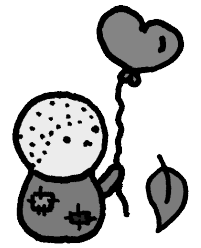
\includegraphics[width=0.15\textwidth]{33bw.png}
\end{wrapfigure}
\begin{itemize}[label=\textbullet, leftmargin=*]
\setlength\itemsep{-0.3em}
\item Est-ce que je coche toujours la même case de genre sur les formulaires ?
\item Serais-je contrarié.e si quelqu’un me désignait par le mauvais genre ?
\item Est-ce que je corrigerais quelqu’un si cette personne m’appelait par un prénom ou un titre erroné ?
\end{itemize}

Cela signifie-t-il pour autant que vous êtes obsédé.e par votre identité ?

Nous pouvons également développer de l’empathie :

\begin{itemize}[label=\textbullet, leftmargin=*]
\setlength\itemsep{-0.3em}
\item Comment me sentirais-je si mon couple était criminalisé par l’État ?
\item Et si je risquais de perdre mon emploi à cause de ma sexualité ou de mon genre ?
\item Ai-je déjà craint d’être attaqué.e pour avoir témoigné de l’affection à quelqu’un en public ?
\item Est-ce que je me battrais pour l’égalité des droits si j’étais traité.e de cette façon ?
\end{itemize}

Indépendamment de notre point de vue sur le soi et le non-soi, la réalité est que les personnes \mbox{LGBTQIA+} continuent d’être victimes d’oppression et de discrimination dans le monde entier. Il s’agit là d’enjeux personnels, sociaux mais aussi spirituels. Faisons en sorte de ne pas perpétuer l’oppression en mettant fin aux discussions sur les problématiques des personnes \mbox{LGBTQIA+} dans nos communautés bouddhistes.

Rappelez-vous également que les bouddhistes sont encouragé.es à développer certains aspects du soi, tels que la générosité, la conduite éthique, la bienveillance, la compassion et la sagesse. Les personnes \mbox{LGBTQIA+} possèdent elles aussi ces qualités.

\begingroup
\begin{figure}[h]
    \centering
    \makebox[0pt]{%
    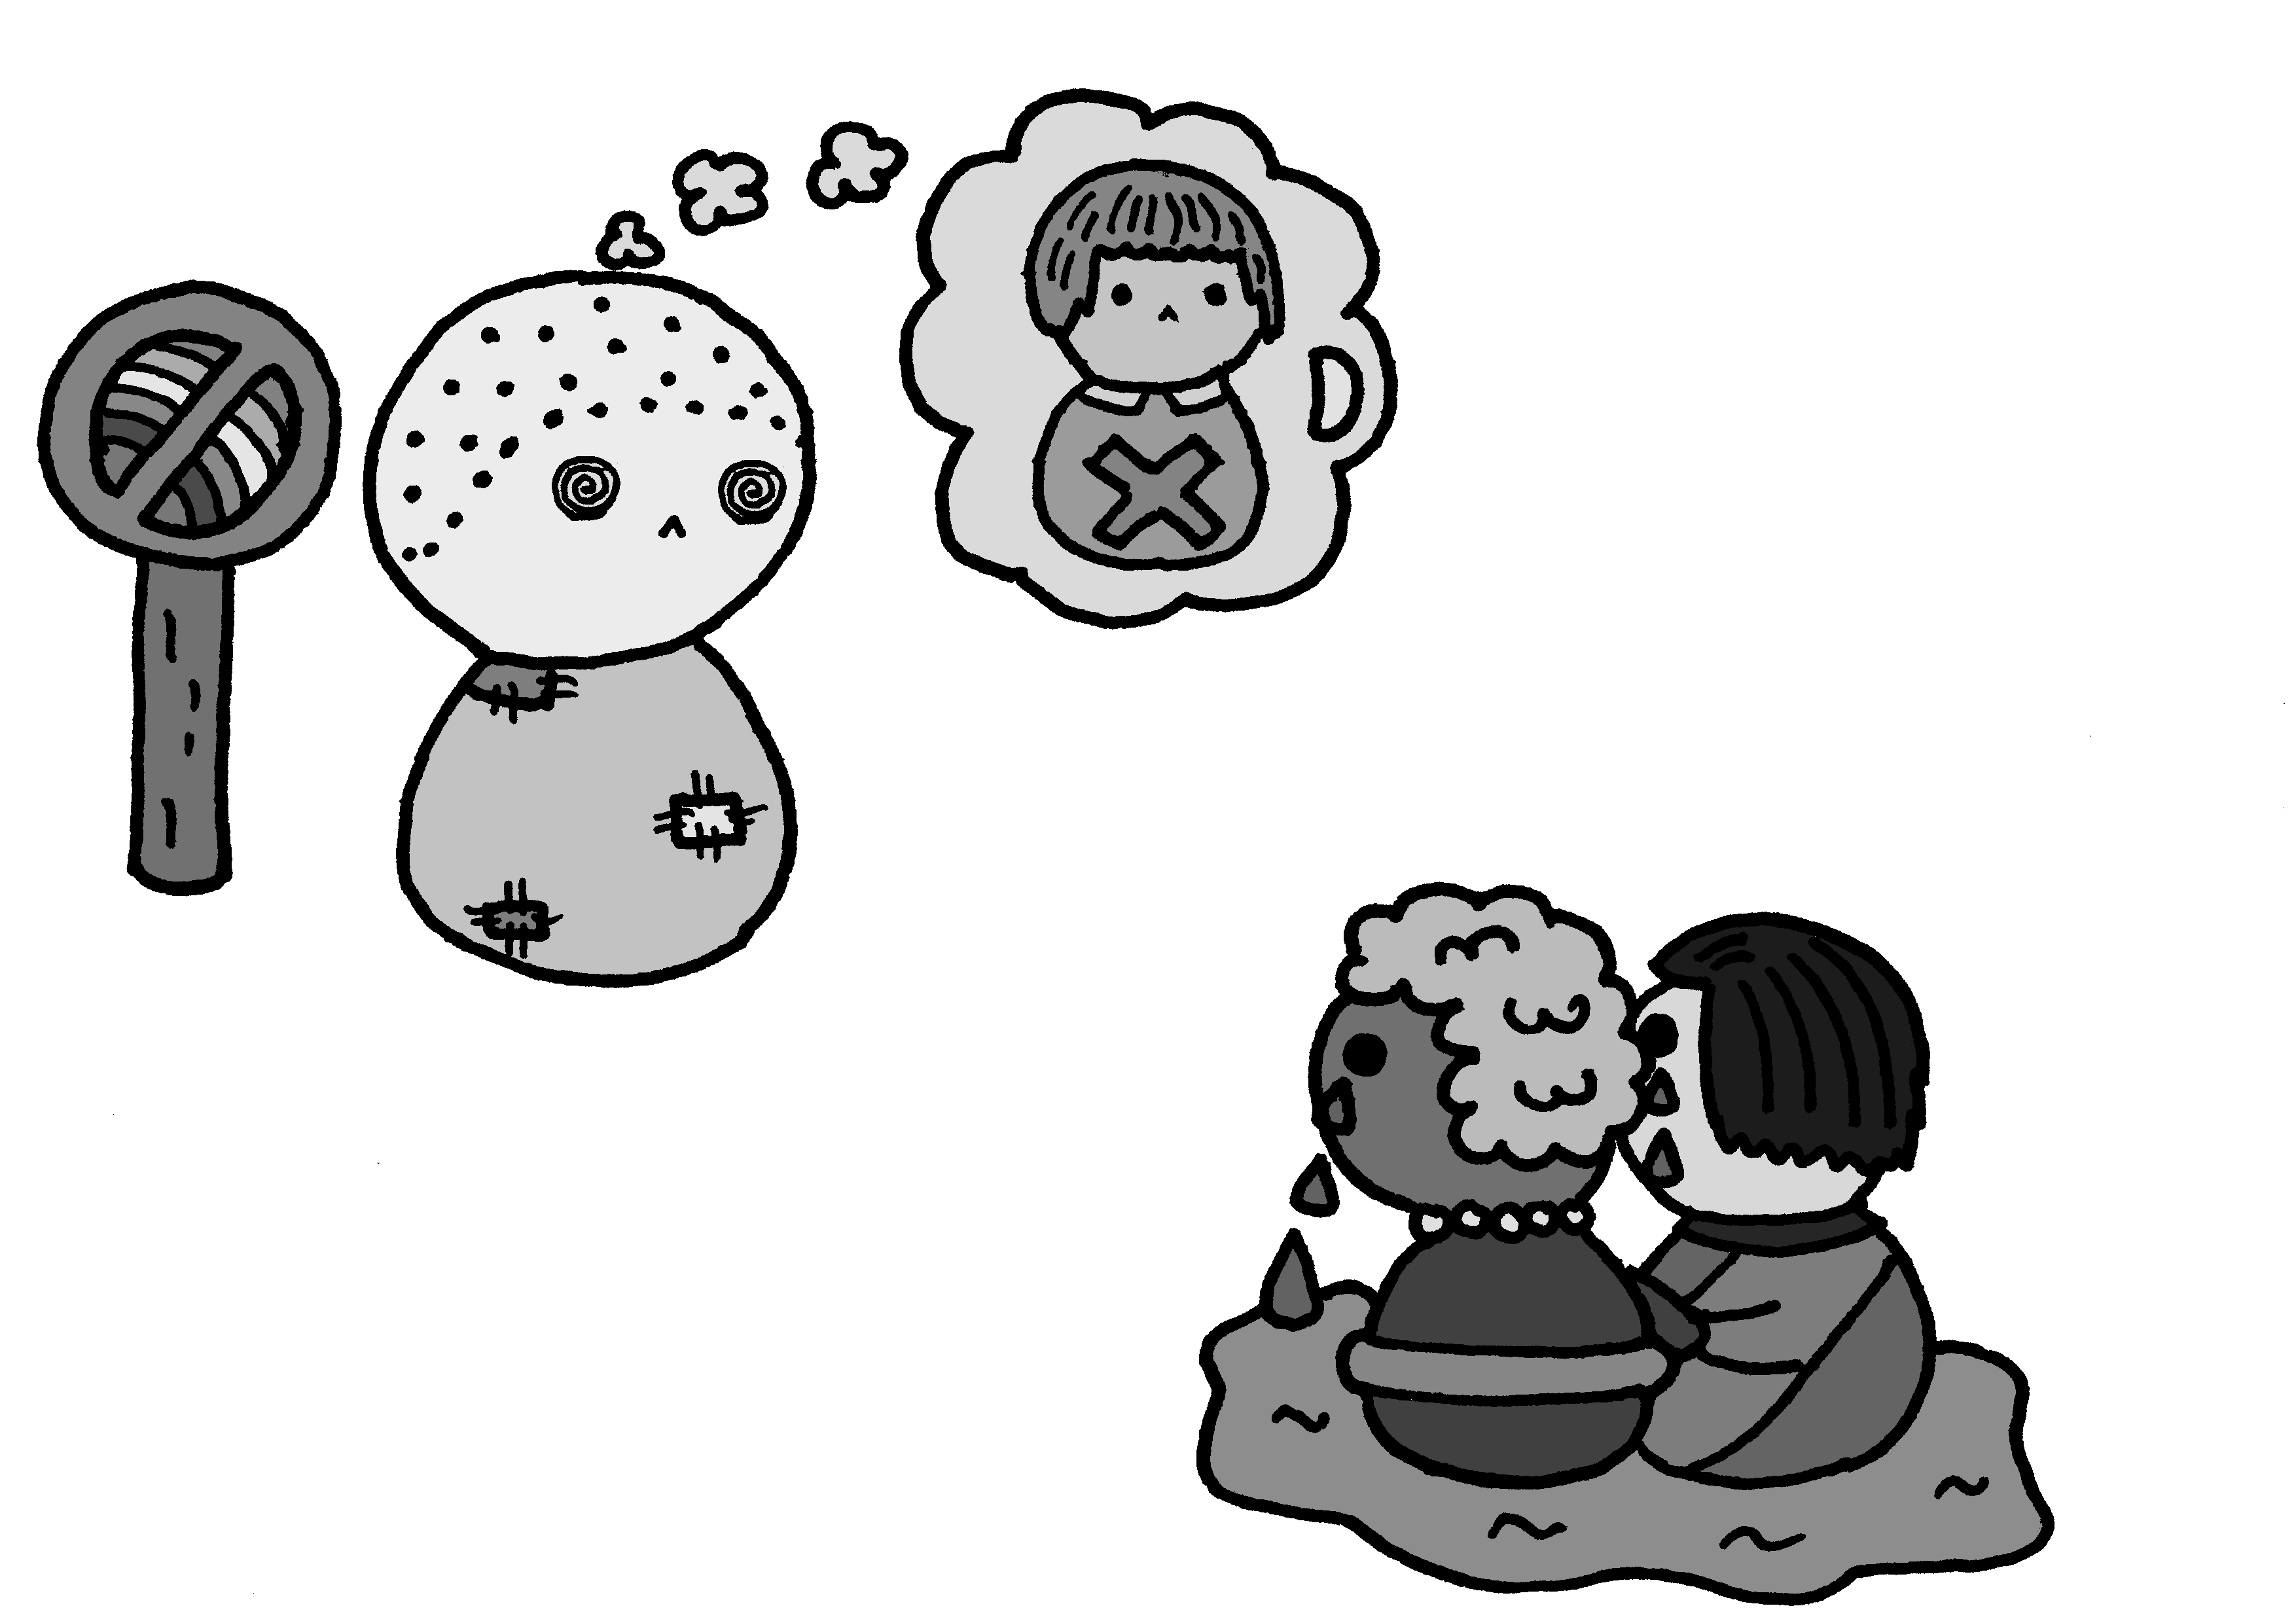
\includegraphics[width=0.3\paperwidth]{30bw.png}}
\end{figure}

\begin{quote}
\doublespacing
\centering
\textit{\Large \textbf{\textcolor{darkgray}{Il est important de reconnaître que nous sommes tout.es différent.es et de comprendre que ces différences comptent.}}}
\end{quote}
\endgroup

\newpage
\phantomsection
\section*{Vécus intersectionnels : \normalsize assignation raciale, genre et \mbox{sexualité}}
\addcontentsline{toc}{section}{Vécus intersectionnels : assignation raciale, genre et sexualité}

\noindent Tout comme les personnes hétérosexuelles et cisgenres, les personnes \mbox{LGBTQIA+}peuvent faire face au racisme, aux préjugés de classe, au validisme et à d’autres types d’idées préconçues. Le terme \mbox{« intersectionnel »} fait référence à un cadre permettant de comprendre comment diverses catégories sociales s’agrègent pour créer des discriminations et des privilèges au sein des sociétés. Cela inclut des catégories sociales telles que l’assignation raciale, le genre, la sexualité, le handicap ou l’absence de handicap, la richesse, le statut économique, la localisation et bien d’autres facteurs encore. Ainsi, une femme transgenre noire qui pratique dans un centre bouddhiste occidental pourrait vivre une expérience très différente de celle d’un homme cisgenre blanc. Ou un homme cis gay asiatique dans un monastère pourrait avoir une expérience différente de celle d’une femme cis hétérosexuelle blanche dans ce même lieu.

Voir les chevauchements entre ces identités nous permet de prendre conscience de la façon dont les discriminations et les privilèges se recoupent pour créer des expériences très différentes, même pour des personnes qui partagent certaines de ces identités. Il est essentiel de comprendre ces différences parce qu’elles nous montrent que les expériences que rencontrent les personnes au sein de la société ne sont pas toutes les mêmes et que des approches diversifiées sont nécessaires pour promouvoir l’inclusion et l’équité pour divers groupes dans nos communautés.

\chapter*{Quelques repères pour mieux comprendre les personnes \mbox{LGBTQIA+}}
\addcontentsline{toc}{chapter}{Quelques repères pour mieux comprendre les personnes \mbox{LGBTQIA+}}
\markboth{Accueillir l’Arc-en-Ciel}{Quelques repères pour mieux comprendre les personnes \mbox{LGBTQIA+}}

\begingroup
\begin{quote}
\centering
\doublespacing
\textit{\large \textbf{\textcolor{darkgray}{Les communautés \mbox{LGBTQIA+} sont très diverses. Elles comptent des individus, des relations, des familles, des amitiés, des sous-cultures et bien plus encore !}}}
\end{quote}
\endgroup

\phantomsection
\section*{Le corps, l’identité de genre et la sexualité sont des choses différentes}
\addcontentsline{toc}{section}{Le corps, l’identité de genre et la sexualité sont des choses différentes}

\noindent Tout le monde a un corps, une identité de genre et une orientation sexuelle. Il est important d’avoir une certaine connaissance de ces concepts de base et de la terminologie qui s’y rapporte pour comprendre les problèmes qui touchent la communauté \mbox{LGBTQIA+}.

\subsubsection*{Le corps et les caractéristiques sexuelles}

\noindent Tous les corps sont différents. Nous avons tou.tes des formes, des tailles et des traits différents. Les corps présentent eux aussi une variété de caractéristiques sexuelles différentes, c’est-à-dire des aspects physiques liés au développement du corps, à la régulation hormonale et aux systèmes reproducteurs. Les principales caractéristiques sexuelles sont les gonades, les chromosomes, les organes génitaux et les hormones.

Les caractéristiques sexuelles secondaires apparaissent à la puberté et peuvent inclure le tissu mammaire, la tonalité de la voix et les poils sur le visage et le pubis. Il est plus exact de parler de \mbox{« c}aractéristiques sexuelle\mbox{s »} que de \mbox{« s}exe biologiqu\mbox{e »}, ou d’utiliser des expressions comme \mbox{« b}iologiquement masculi\mbox{n »} ou \mbox{« b}iologiquement fémini\mbox{n »}, parce que les organes et parties du corps seuls ne sont pas ce qui fait de nous un homme ou une femme. On nous a peut-être appris qu’il n’existe que deux types de corps – le corps masculin et le corps féminin – mais il en existe en réalité une multitude.

\begin{figure}[h]
    \centering
    \makebox[0pt]{%
    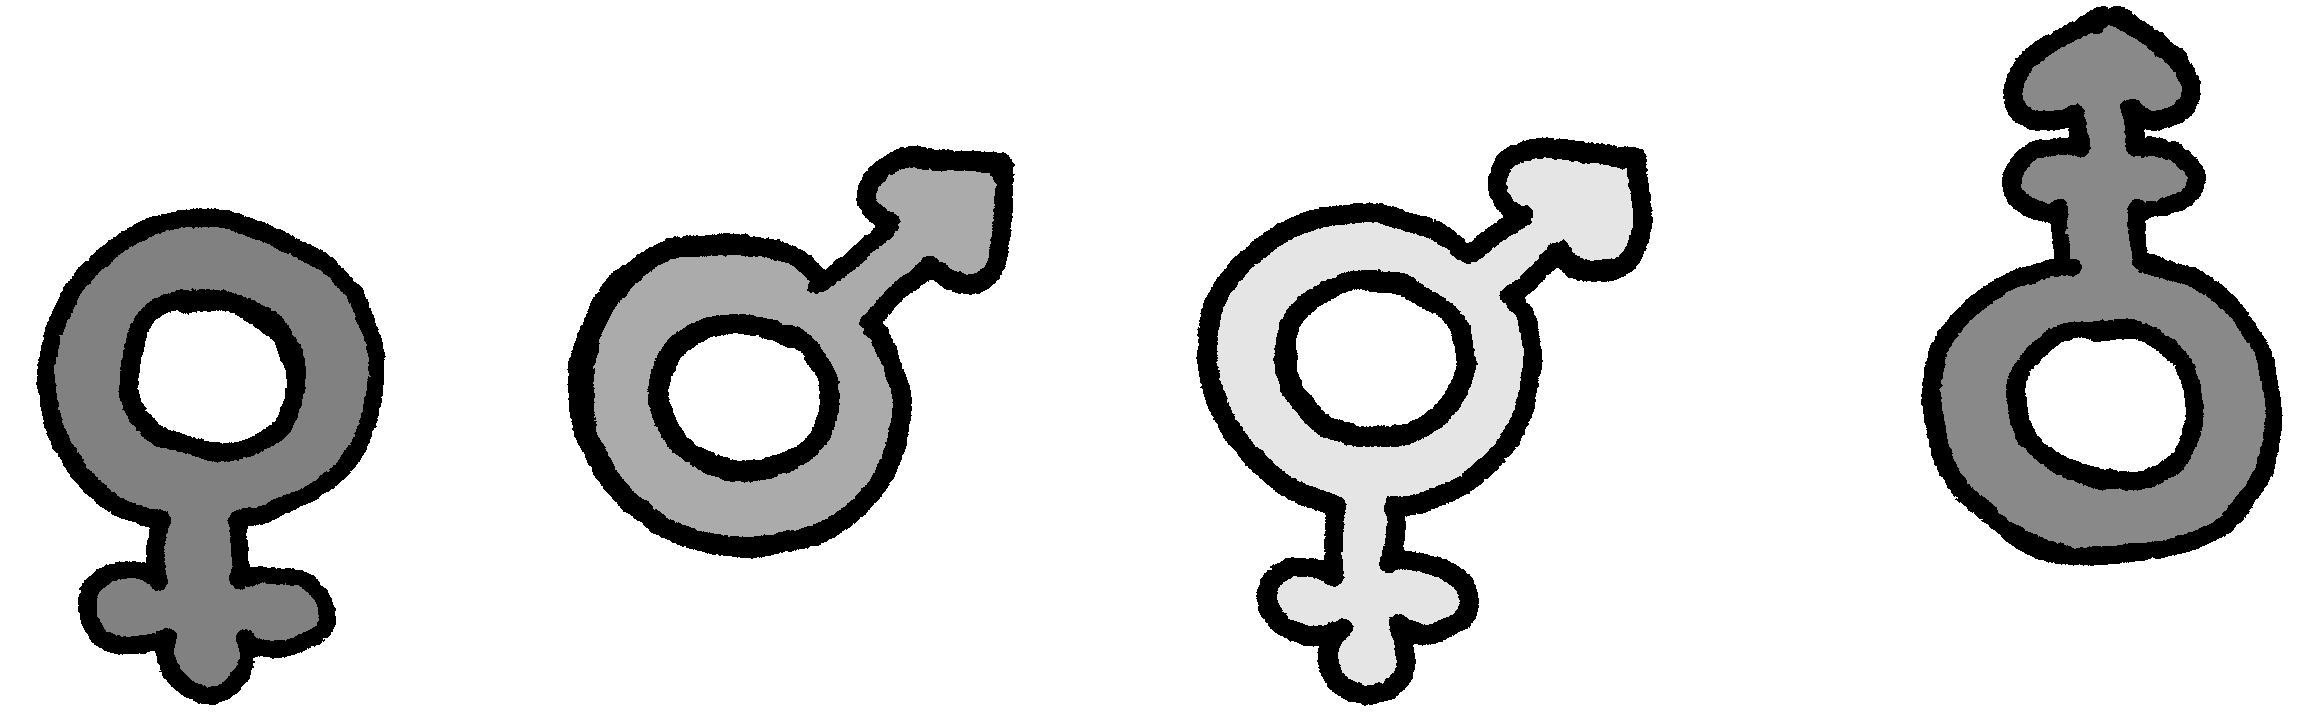
\includegraphics[width=0.17\paperwidth]{38-39bw.png}}
\end{figure}

\subsubsection*{Le corps et le genre}

\noindent Le corps et le genre sont deux choses totalement différentes. Avoir un certain type de corps ne signifie pas que vous devez être d’un certain genre. Une personne de n’importe quel genre peut présenter n’importe quels organes.

L’identité de genre fait partie de notre sentiment intérieur de soi. Le genre peut être féminin, masculin, ni l’un ni l’autre, une combinaison des deux, ou autre chose de tout à fait différent. La relation d’une personne à son genre peut aussi évoluer au fil du temps.

\subsubsection*{Le sexe assigné}

\noindent La plupart d’entre nous se voient attribuer un sexe à la naissance. Cette assignation est renforcée par notre entourage à mesure que nous grandissons. Beaucoup de personnes sont en accord avec le sexe qui leur a été attribué à la naissance, mais ce n’est pas forcément le cas de tout le monde.

\subsubsection*{Cisgenre}

\noindent Le terme \mbox{« cisgenre »} (\mbox{« cis »}, pour faire court) fait référence aux personnes qui s’identifient exclusivement au sexe qui leur a été attribué à la naissance. Par exemple, une personne assignée \mbox{« homme »} à la naissance et qui s’identifie comme un homme est un homme cis.
\mbox{« Cis »} est un terme latin qui signifie \mbox{« d}u même côté qu\mbox{e »}.

\subsubsection*{Transgenre} 

\noindent Le terme \mbox{« transgenre »} (trans, pour faire court) ou \mbox{« d}e genre diver\mbox{s »} décrit les personnes qui ne s’identifient pas exclusivement au sexe qui leur a été assigné à la naissance. Être trans est une question d’identité de genre et de qui nous sommes, et ne concerne pas les personnes vers lesquelles nous sommes attiré.es.

\subsubsection*{L’orientation sexuelle} 

\noindent L’orientation sexuelle, ou sexualité, fait référence aux personnes vers lesquelles nous sommes attiré.es ou non. L’orientation sexuelle n’a rien à voir avec un type de corps ou des caractéristiques sexuelles, ni avec le genre ou l’identité de genre. L’orientation sexuelle est un continuum, et la sexualité de beaucoup de personnes change au fil du temps.

\phantomsection
\section*{Intersexe}
\addcontentsline{toc}{section}{Intersexe}

\noindent \mbox{« Intersexe »} (ou \mbox{« intersexué.e »}) est un terme générique qui décrit les personnes qui présentent naturellement des variations qui s’écartent de l’idée conventionnelle que l’on peut avoir sur les corps \mbox{« féminin »} ou \mbox{« masculin »}. Environ 1,7\% des personnes naissent avec des traits intersexes, qui comprennent un large éventail de caractéristiques génitales, chromosomiques, hormonales et d’autres caractéristiques physiques. Ces caractéristiques peuvent être apparentes au stade prénatal, à la naissance ou se manifester pendant la puberté ou plus tard dans la vie, par exemple lorsque la personne essaie d’avoir un enfant.
Chaque trait a ses propres caractéristiques et différents degrés d’expression. De nombreuses personnes intersexes s’identifient au sexe qui leur a été attribué à la naissance, c’est-à-dire homme ou femme, tandis que d’autres peuvent s’identifier comme \mbox{« autre »}. Certaines personnes intersexes rejettent le sexe qui leur a été assigné à la naissance, mais ne se considèrent pas pour autant comme transgenres. D’autres peuvent s’identifier comme transgenres ou de genre divers. Les personnes intersexes ont la même gamme d’identités que les personnes non intersexes. Certaines s’identifient comme LGBT, mais beaucoup ne le font pas. Être intersexe ne concerne pas l’identité de genre et est différent d’être trans ou non binaire. Cela n’a rien à voir non plus avec l’orientation sexuelle de la personne : les personnes intersexes peuvent être lesbiennes, gays, bisexuelles ou hétérosexuelles, comme n’importe qui d’autre.

\bigskip

\noindent\fbox{%
    \parbox{1.04\textwidth}{%
\textit{\textbf{\Large Attitudes qui nuisent aux personnes intersexes}}

\begin{itemize}[label=\textbullet, leftmargin=*]
\item Vivre dans un monde qui ne reconnaît pas pleinement l’autonomie physique ou les droits humains des personnes intersexes.
\item \mbox{« Gommage »} des caractéristiques divergentes par une chirurgie génitale non consentie dans la petite enfance et par l'administration d’hormones pour faire apparaître les enfants intersexes plus masculins ou féminins.
\item Humiliation sociale et stigmatisation des corps dans l’éducation, les soins de santé, le sport, le travail et d’autres contextes.
\item Utilisation de termes incorrects et obsolètes, comme \mbox{« h}ermaphrodit\mbox{e »}, qui est trompeur et péjoratif, ou qualifier les variations intersexes de \mbox{« troubles »}, alors que ce n’en sont pas.
\end{itemize}
    }%
}

\phantomsection
\section*{Trans et de genre divers}
\addcontentsline{toc}{section}{Trans et de genre divers}

\noindent Les termes \mbox{« trans »} et \mbox{« d}e genre diver\mbox{s »} sont des termes généraux qui décrivent des personnes qui ne s’identifient pas forcément au genre qui leur a été attribué à la naissance. Les personnes transgenres peuvent considérer le fait d’être transgenre comme une histoire ou une expérience plutôt que comme une identité en soi, et considérer leur identité de genre comme étant simplement féminine, masculine ou non binaire. Ou s’identifier spécifiquement comme trans, femme trans ou homme trans. L’expression \mbox{« d}e genre diver\mbox{s »} comprend l’ensemble des différentes manières dont le genre peut être vécu. Elle peut inclure les personnes qui s’identifient comme transgenres ainsi que celles qui s’interrogent sur leur genre. L’expression \mbox{« d}e genre diver\mbox{s »} regroupe également les personnes qui ne s’identifient pas comme hommes ou femmes, telles que les personnes non binaires, ainsi que celles dont le genre tient davantage du continuum. Parmi les termes que certaines personnes utilisent pour décrire le continuum de leur genre, citons \mbox{« genderfluid »}, \mbox{« genderqueer »} et \mbox{« d}e genre non conform\mbox{e »}.

\subsubsection*{Transition ou affirmation de genre}

\noindent La transition ou l’affirmation de genre désigne le fait qu’une personne prend des mesures pour se sentir socialement ou physiquement plus alignée avec son identité de genre. Il s’agit d’un processus personnel qui semble adéquat pour pouvoir vivre son genre au sein de la société. La transition peut passer par des mesures sociales, médicales, chirurgicales et juridiques visant à affirmer le genre d’une personne. La transition ne signifie pas que quelqu’un \mbox{« c}hange de genr\mbox{e »} ou \mbox{« c}hange de sex\mbox{e »} ou \mbox{« devient »} un homme ou une femme, mais plutôt que cette personne affirme le genre qu’elle a toujours eu. Le parcours de chaque personne trans est différent ; il n’y a pas de \mbox{« t}ransition complèt\mbox{e »}, en ce sens que la transition de chaque personne est complète en soi, à sa manière, indépendamment de son apparence, de ce que disent ses documents, de ses hormones ou des interventions chirurgicales qu’elle a subies ou non. Ce processus de transition ne revient pas à s’identifier en tant que trans. Certaines personnes qui effectuent cette transition peuvent toujours s’identifier comme trans, mais d’autres s’identifieront simplement comme homme ou femme.

\subsubsection*{Transition sociale}

\noindent Il s’agit du processus par lequel une personne modifie son expression de genre afin de mieux la faire correspondre à son identité de genre. Elle peut par exemple s’affirmer comme personne trans, ou changer son nom et ses pronoms, son apparence. Il se peut aussi que la personne change la façon dont elle interagit dans les espaces genrés et, par exemple, n’utilise plus les mêmes toilettes. La transition sociale peut également supposer de faire changer la mention de son sexe sur un passeport, un certificat de naissance et d’autres documents.

\subsubsection*{Transition physique}

\noindent Ce processus de transition suppose de modifier son apparence corporelle, et par exemple ses vêtements, son maquillage et ses cheveux, pour qu’ils correspondent à son identité de genre, ou de demander un traitement médical tel que des hormones ou une intervention chirurgicale.

\subsubsection*{Non binaire}

\noindent Le terme \mbox{« n}on binair\mbox{e »}, ou \mbox{« NB »}, relève de la catégorie \mbox{« trans »}. « Non binaire » est un terme utilisé pour décrire les personnes qui

\noindent\fbox{%
    \parbox{1.02\textwidth}{%
\textit{\textbf{\Large Attitudes qui nuisent aux personnes trans et non binaires}}

\medskip

Le cissexisme/cisgenrisme est une vision sociale discriminatoire qui prétend que l’identité trans n’existe pas. Ce point de vue préjudiciable soutient que seules les identités binaires (masculines ou féminines) sont valables ou réelles, et que l’identité de genre est fixée à la naissance et se fonde exclusivement sur les caractéristiques sexuelles.

Le mégenrage consiste à décrire une personne ou à s’adresser à elle en des termes qui ne correspondent pas à son identité de genre. Cela comprend, par exemple, l’utilisation de pronoms impropres (elle, il, iel), de titres familiaux inadéquats (père, soeur, oncle) ou encore d’autres mots qui ont traditionnellement des connotations genrées, telles que jolie, etc. 

La transphobie fait référence aux préjugés et stéréotypes négatifs sur les personnes trans et de genre divers. La transphobie comprend, par exemple, un langage irrespectueux ou insultant vis-à-vis de ces personnes ou une propension à restreindre la façon dont les personnes sont autorisées à exprimer leur identité de genre à travers leurs vêtements, les toilettes qu’elles décident de fréquenter ou la formule d’hébergement qu’elles choisissent. 

La transphobie inclut aussi les menaces, les violences physiques et verbales, le harcèlement sexuel et l’exclusion d’une personne en raison de son identité de genre.
    }%
}

\newpage
\noindent ne s’identifient pas comme homme ou femme. Celles-ci peuvent estimer qu’elles incarnent des éléments des deux, ou qu’elles se situent quelque part entre les deux, ou encore qu’elles sont tout autre chose. Les personnes non binaires peuvent cependant avoir un sens aigu de leur genre. Il peut être très pénible pour elles de s’entendre dire qu’elles doivent s’identifier comme homme ou femme. Une personne peut s’identifier uniquement comme non binaire ou se référer au terme \mbox{« n}on binair\mbox{e »} comme à un terme générique recouvrant diverses expériences de genre non binaires. Les termes regroupés sous ce générique incluent \mbox{« genderfluid »}, \mbox{« genderqueer »} (qui connaît un continuum de genre), \mbox{« t}rans-masculi\mbox{n »} et \mbox{« t}rans-fémini\mbox{n »} (personne non binaire mais penchant davantage du côté d’un genre), \mbox{« agenre »} (n’ayant pas de genre) et \mbox{« bigenre »} (qui s’identifie à la fois comme homme et comme femme). Ces termes , et d’autres, décrivent le ressenti des personnes NB vis-à-vis de leur genre et de son expression. De nombreuses personnes non binaires s’identifient également comme transgenres. Être non binaire ne signifie pas être intersexe. La plupart des personnes non binaires naissent avec des corps conventionnellement masculins ou féminins, mais grandissent avec le sentiment d’être différentes. Être non binaire n’a rien à voir avec l’orientation sexuelle : les personnes non binaires peuvent avoir la même gamme d’orientations que les autres. Certaines personnes non binaires choisissent de subir une intervention chirurgicale ou de prendre des hormones pour modifier leur corps et se sentir plus à l’aise. D’autres n’en veulent pas et sont heureuses avec leur corps tel qu’il est. Certaines personnes non binaires se présentent de manière androgyne, tandis que d’autres ont l’air conventionnellement masculines ou féminines, tout en n’en étant pas moins non binaires.

\phantomsection
\section*{Orientation sexuelle}
\addcontentsline{toc}{section}{Orientation sexuelle}

\noindent Le genre et l’orientation sexuelle sont deux choses différentes. Le genre est la façon dont nous nous voyons, et cela peut être comme une femme, comme un homme, comme un mélange des deux, ou comme tout autre chose. L’orientation sexuelle a trait à notre attirance. Une personne cisgenre peut être gay, hétérosexuelle, bisexuelle ou asexuelle. Une personne trans peut aussi être hétérosexuelle, bisexuelle, asexuelle, gay ou avoir toute autre orientation sexuelle.

\subsubsection*{Lesbienne}

\noindent Une personne qui s’identifie comme femme et est attirée sexuellement et/ou romantiquement par d’autres personnes qui s’identifient comme femmes.

\subsubsection*{Gay}

\noindent Une personne qui s’identifie comme homme et est attirée sexuellement et/ou romantiquement par d’autres personnes qui s’identifient comme hommes.

\subsubsection*{Queer}

\noindent Décrit toute une gamme d’orientations sexuelles et d’identités de genre. Autrefois utilisé comme un terme péjoratif, \mbox{« queer »} a été récupéré et est maintenant souvent utilisé comme un terme générique pour décrire l’ensemble des identités LGBTIQA+.

\subsubsection*{Bisexuelle}

\noindent Une personne qui est attirée sexuellement et/ou romantiquement par des personnes du même genre ainsi que par des personnes d’un autre genre. La bisexualité ne suppose pas nécessairement qu’il n’y ait que deux genres, et le terme pansexuel s’est développé pour inclure spécifiquement une attirance non limitée par le genre, \mbox{y compris l’attirance pour les personnes trans et non binaires}.

\subsubsection*{Hétérosexuelle}

\noindent Une personne attirée sexuellement et/ou romantiquement par le sexe opposé.

\subsubsection*{Orientation romantique}

\noindent Décrit l’attirance sur le plan romantique. Cette attirance peut être distincte de notre orientation sexuelle. Les orientations romantiques fonctionnent globalement de la même manière que les orientations sexuelles et décrivent le(s) genre(s) par le(s)quel(s) la personne est attirée.

\subsubsection*{Asexuelle}

\noindent Orientation sexuelle définie par l’absence d’attirance sexuelle, que ce soit dans le cadre de relations ou en dehors de celles-ci. Les personnes asexuelles peuvent éprouver une attirance romantique dans le continuum \mbox{LGBTQIA+} et avoir des relations sexuelles, même si elles n’éprouvent pas d’attirance sexuelle.

\bigskip

\noindent\fbox{%
    \parbox{1.02\textwidth}{%
\textit{\textbf{\Large Attitudes qui nuisent aux personnes attirées par le même sexe}}

\medskip

\textbf{Biphobie}: attitude préjudiciable envers une personne attirée par plus d’un genre. Par exemple dire à une personne que sa sexualité n’est \mbox{« q}u’une phas\mbox{e »} ou l’enjoindre de \mbox{« c}hoisir un cam\mbox{p »}. Étiqueter les personnes bisexuelles comme homosexuelles ou hétérosexuelles parce qu’elles vivent une relation donnée revient à invisibiliser leur véritable identité bisexuelle.

\medskip

\textbf{Hétéronormativité}: l’opinion selon laquelle les relations hétérosexuelles sont les seules expressions naturelles, normales et légitimes de la sexualité et des relations, et que les autres sexualités ou identités de genre sont contre-nature et constituent une menace pour la société.

\medskip

\textbf{Homophobie}: croyances, préjugés et stéréotypes négatifs sur les personnes non hétérosexuelles. L’homophobie verbale en est une forme courante et regroupe entre autres les insultes, les rumeurs et les propos injurieux (\mbox{« pédé »} ou \mbox{« gouine »}) ou des phrases comme \mbox{« c}’est tellement ga\mbox{y »}. L’homophobie désigne également les menaces, les violences physiques et verbales, le harcèlement sexuel, les mesures législatives discriminatoires et l’exclusion délibérée d’une personne en raison de sa sexualité.
    }%
}

\newpage
\textbf{Plus d'informations: }https://rainbodhi.org/resources/

\medskip

{\footnotesize
\begin{center}
\noindent \textbf{Version originale 2021:} 

This booklet was produced by \mbox{LGBTQIA+} Buddhists. All identity groups in the rainbow acronym were consulted for input and feedback.

\noindent Many thanks to Venerable Vimala, Ayya Vimalanyani, Bhante Sumano, Erland Moeckli, JJ, Nilushi Disayanake, Letty, all the Rainbodhi crew, the Buddhist Council of NSW, GiveOUT Day Australia, Simone Ford, Bronwyn Sweeney and a special thanks to all the many people who donated funds to produce this booklet.

\medskip

\noindent First Published in Australia 2021 by MegaCity Books for Rainbodhi \mbox{LGBTQIA+} Buddhist Community

\smallskip


\includegraphics{by-nc-sa}

\noindent This work is created under a Creative Commons Attribution-NonCommercial-ShareAlike 4.0 International License

\noindent A catalogue record for this book is available from the National Library of Australia.

\medskip

\noindent ISBN: I978-0-64889593-1-1

\medskip

Author: Akāliko Bhikkhu \\
Illustrator: Venerable Yodha \\
Contributor: Letty \\
Project management and design: Kerry Klinner, megacitydesign.com \\
Editor: Simone Ford \\
Proofreader: Bronwyn Sweeney

\bigskip

\textbf{Édition française 2023:}  \\
Traduction: Francoise Leclercq, Jessica Hefes \\
Relecture: Mokushō Deprèay, Grégory Renders \\
Illustrations : Vénérable Yodha \\
Mise en page de l'édition imprimée : Remy Jakobson
\end{center}
}

\newgeometry{margin=0pt}

\begin{figure}[ht]
    \centering
    \makebox[0pt]{%
    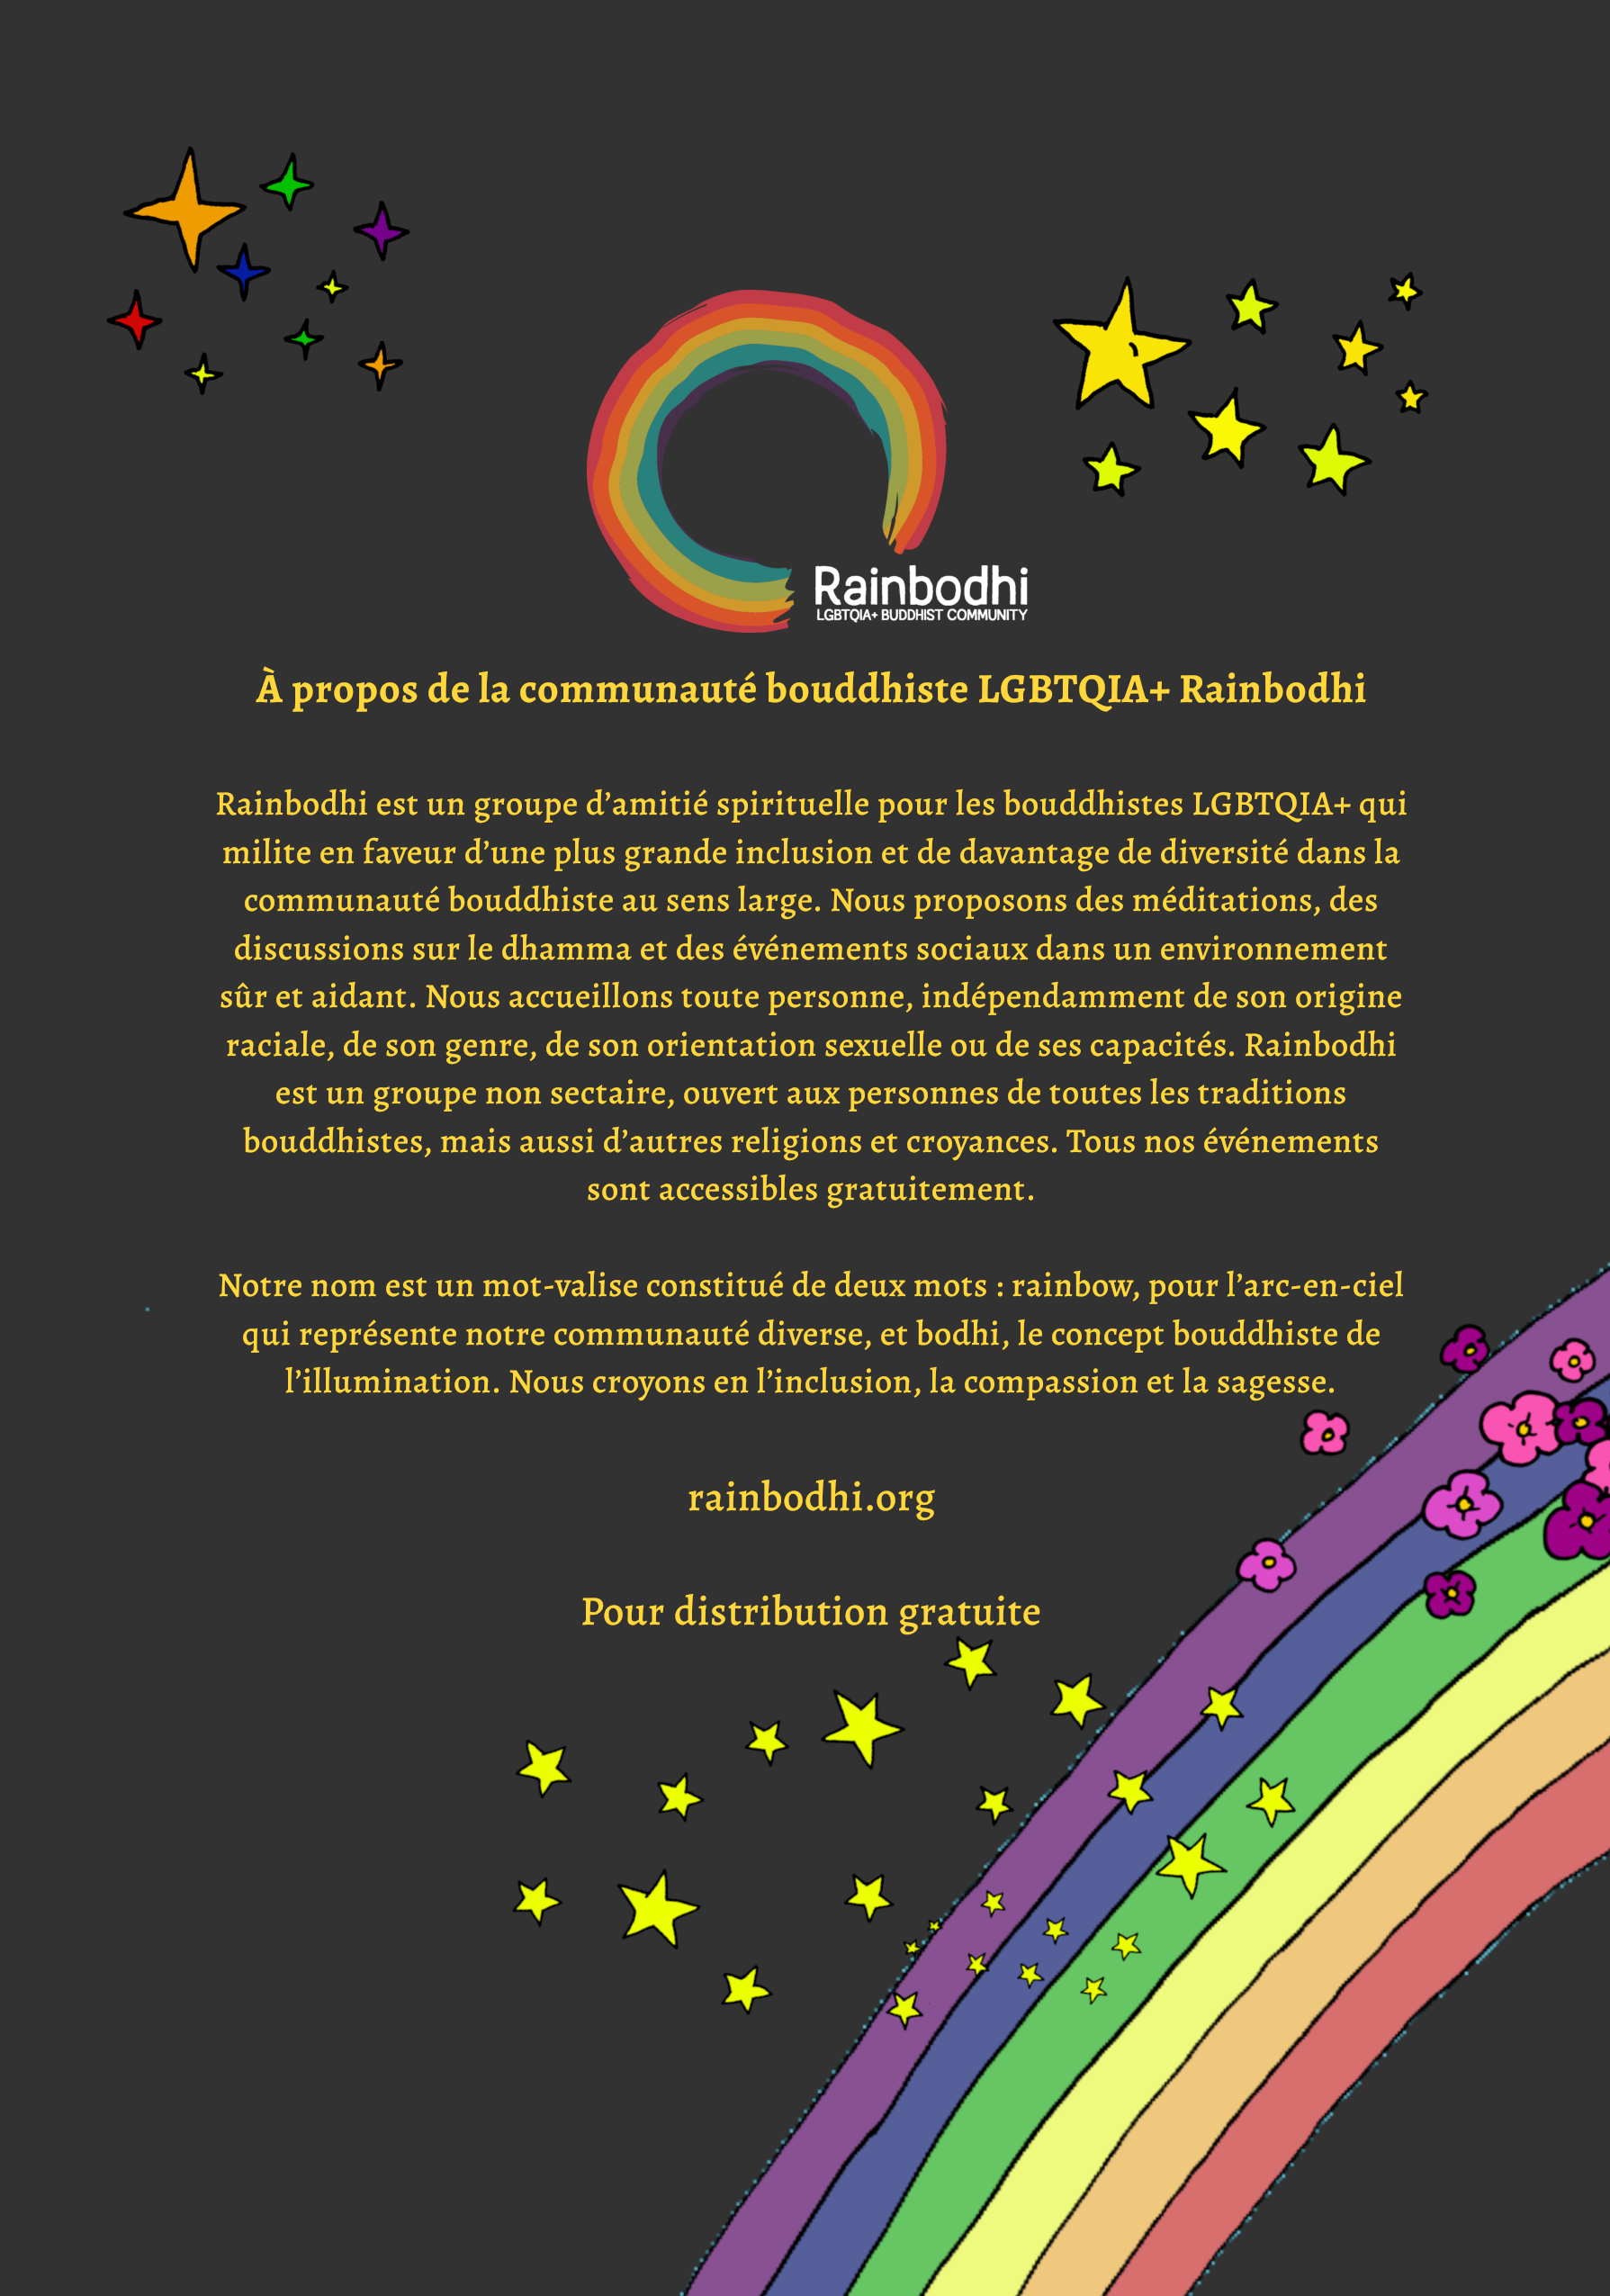
\includegraphics[width=\paperwidth]{back_francais}}
\end{figure}

\end{document}
